\documentclass[11pt,a4paper]{article}

% ── packages ──────────────────────────────────────────────────────────────────
\usepackage[margin=2.2cm,top=2.3cm,bottom=2.2cm]{geometry}
\usepackage{graphicx}
\usepackage{booktabs}
\usepackage{longtable}
\usepackage{amsmath,amssymb}
\usepackage{hyperref}
\usepackage{xcolor}
\usepackage{float}
\usepackage{enumitem}
\usepackage{caption}
\usepackage{subcaption}
\usepackage{titlesec}
\usepackage{fancyhdr}
\usepackage{parskip}
\usepackage[utf8]{inputenc}
\usepackage[T1]{fontenc}
\usepackage{lmodern}
\usepackage{multicol}
\usepackage{tabularx}

% ── compact spacing ──────────────────────────────────────────────────────────
\setlength{\parskip}{2pt plus 1pt minus 1pt}
\setlength{\parindent}{0pt}
\setlength{\floatsep}{6pt plus 2pt minus 2pt}
\setlength{\textfloatsep}{8pt plus 2pt minus 2pt}
\setlength{\intextsep}{6pt plus 2pt minus 2pt}
\setlength{\abovecaptionskip}{4pt}
\setlength{\belowcaptionskip}{2pt}
\captionsetup{font=small,labelfont=bf}
\setlist{nosep,topsep=2pt,parsep=1pt}

\hypersetup{
    colorlinks=true,
    linkcolor=blue!60!black,
    citecolor=blue!60!black,
    urlcolor=blue!60!black,
}

\pagestyle{fancy}
\fancyhf{}
\fancyhead[L]{\small Credit Risk Modelling --- DSL Course Project}
\fancyhead[R]{\small IIT Kharagpur}
\fancyfoot[C]{\thepage}

\titleformat{\section}{\large\bfseries}{\thesection}{0.7em}{}[\vspace{-0.6em}\rule{\textwidth}{0.4pt}]
\titleformat{\subsection}{\normalsize\bfseries}{\thesubsection}{0.5em}{}
\titleformat{\subsubsection}{\small\bfseries}{\thesubsubsection}{0.5em}{}
\titlespacing*{\section}{0pt}{8pt plus 2pt minus 2pt}{4pt plus 1pt minus 1pt}
\titlespacing*{\subsection}{0pt}{6pt plus 2pt minus 1pt}{2pt plus 1pt}
\titlespacing*{\subsubsection}{0pt}{4pt plus 1pt}{2pt}
\titlespacing*{\paragraph}{0pt}{3pt plus 1pt}{0.5em}

\graphicspath{{img/}}

% ══════════════════════════════════════════════════════════════════════════════
\begin{document}

% ── title page ────────────────────────────────────────────────────────────────
\begin{titlepage}
\centering
\vspace*{0.5cm}

\includegraphics[width=3.5cm]{img/iitkgp_logo.jpeg}\par
\vspace{0.5cm}
{\Large\bfseries INDIAN INSTITUTE OF TECHNOLOGY KHARAGPUR\par}
\vspace{0.2cm}
{\normalsize Data Science Lab (DSL) --- Course Project Report\par}
\vspace{1.2cm}
{\LARGE Credit Risk Modelling:\par}
\vspace{0.3cm}
{\normalsize An Explainable Credit Scoring System: Integrating Default Probability\\
Estimation with CIBIL Score Calculation and Borrower Guidance\par}
\vspace{1cm}
\rule{\textwidth}{0.4pt}
\vspace{1cm}
{\normalsize Under the guidance of: \textbf{Swaminathan Rammohan}\par}
\vspace{1cm}
{\normalsize Submitted by:\par}
\vspace{0.3cm}
\begin{tabular}{l@{\hspace{1.2cm}}l}
Hrishav Majumdar & 25BM6JP15 \\
Kingshuk Barua & 25BM6JP23 \\
Patil Rohit Ranjit & 25BM6JP34 \\
Pritam Sarkar & 25BM6JP40 \\
Siddharth Sharan & 25BM6JP48 \\
\end{tabular}
\vspace{1cm}
{\normalsize April 2026\par}
\end{titlepage}

% ── abstract ──────────────────────────────────────────────────────────────────
\section*{Abstract}
\addcontentsline{toc}{section}{Abstract}

\small
This report presents an ML-driven credit risk modelling framework for Indian banks and NBFCs. Using the ``Give Me Some Credit'' dataset (150K borrower records, 11 features), we train Logistic Regression, XGBoost, CatBoost, and a Mixture-of-Experts (MoE) neural network. CatBoost, optimised via Optuna (50 TPE trials), achieves ROC-AUC~$\approx$~0.86. A dual-threshold framework (Max-F1 and Precision-targeted) enables calibrated precision--recall trade-offs. SHAP provides per-feature explanations with actionable recommendations. A CIBIL-aligned score (300--900) weights default probability at 50\%, payment history 25\%, credit utilisation 15\%, credit mix 10\%. Deployed via Next.js CRM dashboard and Google Sheets API.
\normalsize

\subsection*{Summary of Contributions}
\small
\begin{itemize}[nosep]
    \item Thorough EDA through univariate, bivariate plots, and correlation analysis using statistical methods: Point-biserial~$r$, Mann-Whitney~$U$, Rank-biserial~$r$, Cohen's~$d$, AUC (continuous vs binary) and $\chi^2$, Cram\'{e}r's~$V$, Odds Ratio, Cochran-Armitage trend, Somers'~$D$ (discrete vs binary).
    \item Built a production-grade credit risk engine combining gradient boosting (CatBoost) and neural MoE models plus distillation, achieving $\sim$0.86 ROC-AUC and enabling probabilistic risk scoring.
    \item Developed and benchmarked 4 model architectures (Logistic Regression, XGBoost, CatBoost, Mixture-of-Experts), improving performance over baseline by $\sim$4\% AUC.
    \item Designed a dual-threshold decision framework (Max-F1 \& Precision-constrained) enabling flexible risk calibration for different business scenarios.
    \item Identified key business insights such as delinquency features as dominant predictors and importance of threshold selection over model choice.
    \item Built a production-ready ML pipeline with modular architecture (data preprocessing, training, evaluation, deployment) ensuring scalability and reproducibility.
    \item Integrated model explainability (SHAP) into predictions, translating black-box outputs into actionable borrower-level insights.
    \item Deployed an end-to-end ML system (Python + React) enabling real-time inference and scalable batch processing.
\end{itemize}
\normalsize

\newpage
\tableofcontents
\newpage

% ══════════════════════════════════════════════════════════════════════════════
\section{Introduction}

Credit risk assessment is critical in Indian financial services (INR~150 lakh crore disbursed by FY~2024--25; gross NPAs $\approx$~2.8\%). The current landscape suffers from:
\begin{itemize}
    \item \textbf{Static scorecards} that miss non-linear interactions.
    \item \textbf{Opaque decisions} without actionable borrower explanations.
    \item \textbf{Reactive posture} --- point-in-time rather than predictive.
    \item \textbf{Threshold rigidity} --- single boundary instead of calibrated trade-offs.
\end{itemize}
This project develops an ML-driven framework combining predictive accuracy with SHAP-based explainability, CIBIL-aligned scoring, and real-time deployment.


% ══════════════════════════════════════════════════════════════════════════════
\section{Dataset Description}

The project uses the ``Give Me Some Credit'' dataset containing 150,000 training observations with 11 financial attributes.

\begin{table}[H]
\centering\small
\caption{Feature descriptions}
\begin{tabular}{@{}llll@{}}
\toprule
\textbf{Kaggle Name} & \textbf{Internal Name} & \textbf{Type} & \textbf{Description} \\
\midrule
SeriousDlqin2yrs & \texttt{defaulted} & Binary & Target: 90+ days past due in 2~yr \\
RevolvingUtilization\ldots & \texttt{unsecured\_credit} & Float & Revolving utilisation ratio \\
age & \texttt{age} & Integer & Borrower age in years \\
NumberOfTime30--59\ldots & \texttt{delinq\_30\_59} & Count & 30--59 day late payments \\
DebtRatio & \texttt{debt\_ratio} & Float & Monthly debt / income \\
MonthlyIncome & \texttt{monthly\_income} & Float & Monthly salary (USD) \\
NumberOfOpenCredit\ldots & \texttt{open\_credit} & Count & Open credit lines \\
NumberOfTimes90DaysLate & \texttt{delinq\_90} & Count & 90+ day late events \\
NumberRealEstate\ldots & \texttt{real\_estate\_loans} & Count & Home/mortgage loans \\
NumberOfTime60--89\ldots & \texttt{delinq\_60\_89} & Count & 60--89 day late payments \\
NumberOfDependents & \texttt{dependents} & Count & Household dependents \\
\bottomrule
\end{tabular}
\end{table}

\textbf{Key statistics}: 150,000 rows $\rightarrow$ \textbf{112,021} after cleaning. Default rate: 6.74\% ($\approx$~13.5:1 class imbalance). Values 96 and 98 in delinquency fields are sentinel codes (not actual counts).


% ══════════════════════════════════════════════════════════════════════════════
\section{Data Cleaning \& Preprocessing Pipeline}

Shared across all notebooks:
\begin{enumerate}
    \item \textbf{Column rename}: Kaggle names $\to$ snake\_case.
    \item \textbf{Remove age $\leq$ 0}: Impossible ages filtered out.
    \item \textbf{Sentinel flag}: \texttt{delinq\_90} $\in \{96, 98\}$ $\to$ \texttt{delinq\_sentinel = 1} (54.6\% default rate vs 6.6\%).
    \item \textbf{Delinquency cap}: All delinq columns clipped to $\leq 10$.
    \item \textbf{Missing indicators}: \texttt{monthly\_income\_missing} (19.8\% MNAR), \texttt{dependents\_missing} (2.6\% MCAR).
    \item \textbf{Median imputation}: Income and dependents filled with column median.
    \item \textbf{Train/Val/Test split}: 70/15/15\% stratified.
\end{enumerate}
Final: 13 features (10 original + 3 engineered).


% ══════════════════════════════════════════════════════════════════════════════
\section{Exploratory Data Analysis}

\subsection{Sentinel Accounts \& Missingness}

Two key data-quality findings emerge before any modelling:

\paragraph{Sentinel codes in delinquency fields.}
Values 96 and 98 in the delinquency columns are data-entry codes, not actual past-due counts.
Only 269 accounts (0.18\%) carry these codes, but they exhibit a \textbf{54.6\% default rate} vs.\ 6.6\% for non-sentinel borrowers --- an 8$\times$ difference.
We retain these rows, flag them with \texttt{delinq\_sentinel = 1}, and cap all delinquency counts at 10.

\begin{figure}[H]
\centering
\begin{subfigure}[b]{0.65\textwidth}
    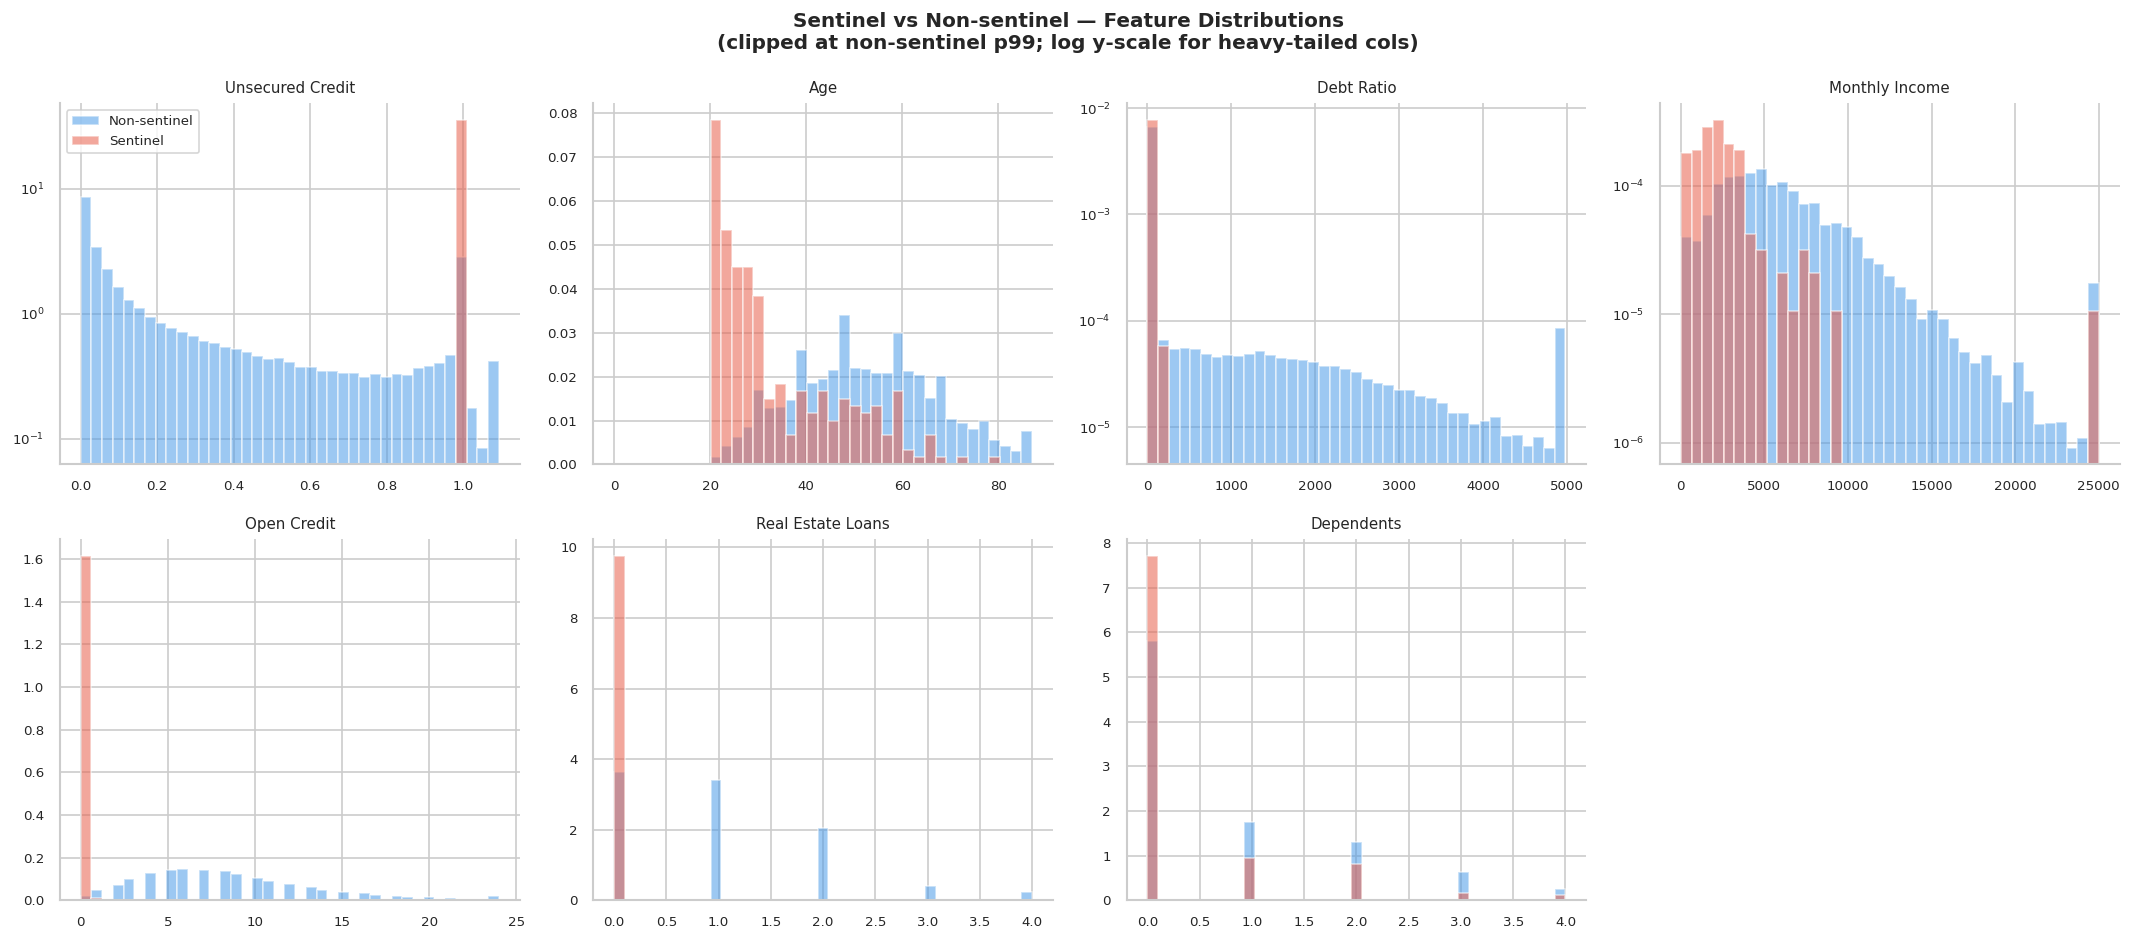
\includegraphics[width=\textwidth]{eda/eda_cell010_out000.png}
    \caption{Feature distributions: sentinel (red) vs non-sentinel (blue)}
\end{subfigure}
\hfill
\begin{subfigure}[b]{0.30\textwidth}
    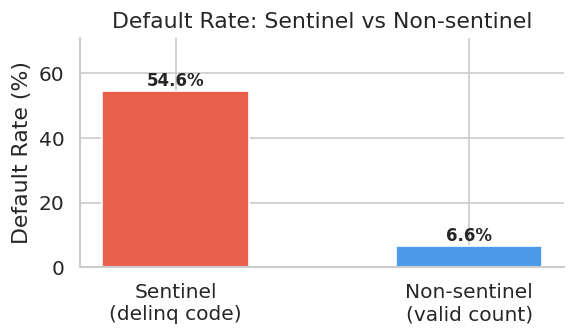
\includegraphics[width=\textwidth]{eda/eda_cell010_out001.png}
    \caption{Default rate comparison}
\end{subfigure}
\caption{Sentinel vs non-sentinel account profiles}
\end{figure}

Sentinel borrowers are younger (median age 33 vs 52), have near-maximal credit utilisation, and carry substantially lower incomes --- a high-risk profile consistent with the extreme default rate.

\paragraph{Missing values.}
Only two columns have missing data:

\begin{table}[H]
\centering\small
\caption{Missing value summary}
\begin{tabular}{@{}lrrl@{}}
\toprule
\textbf{Column} & \textbf{Missing} & \textbf{\%} & \textbf{Mechanism} \\
\midrule
\texttt{monthly\_income} & 29,731 & 19.8\% & MNAR --- missing borrowers default less (5.6\% vs 6.9\%) \\
\texttt{dependents}      &  3,924 &  2.6\% & MCAR --- no association with target \\
\bottomrule
\end{tabular}
\end{table}

The counter-intuitive finding that missing income is \emph{protective} suggests MNAR: financially stable borrowers (self-employed, investment income) are less likely to report salaried income.
Binary indicators \texttt{monthly\_income\_missing} and \texttt{dependents\_missing} are created before median imputation to preserve this signal.

\subsection{Univariate Analysis --- Continuous Features}

Histograms with KDE overlays reveal extreme right-skew in \texttt{monthly\_income}, \texttt{debt\_ratio}, and \texttt{unsecured\_credit}. Log1p transforms are applied for visualisation and for linear/neural models.

\begin{figure}[H]
\centering
\begin{subfigure}[b]{0.48\textwidth}
    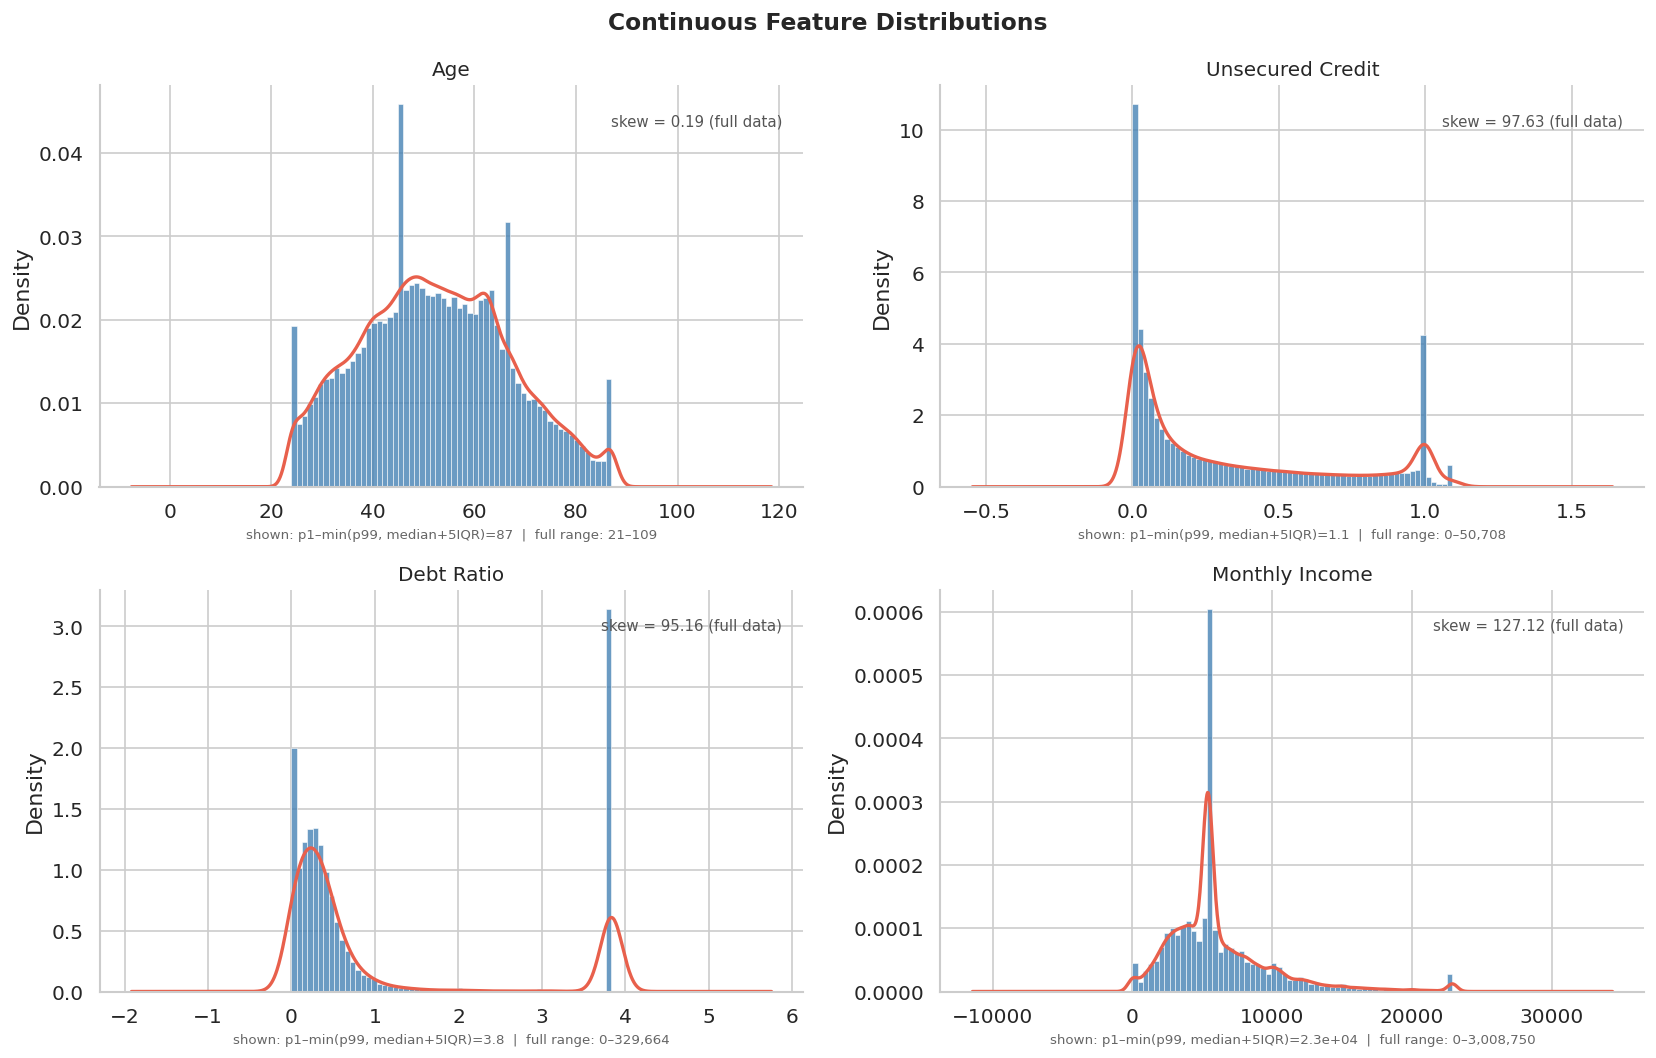
\includegraphics[width=\textwidth]{eda/eda_cell018_out000.png}
    \caption{Continuous feature distributions}
\end{subfigure}
\hfill
\begin{subfigure}[b]{0.48\textwidth}
    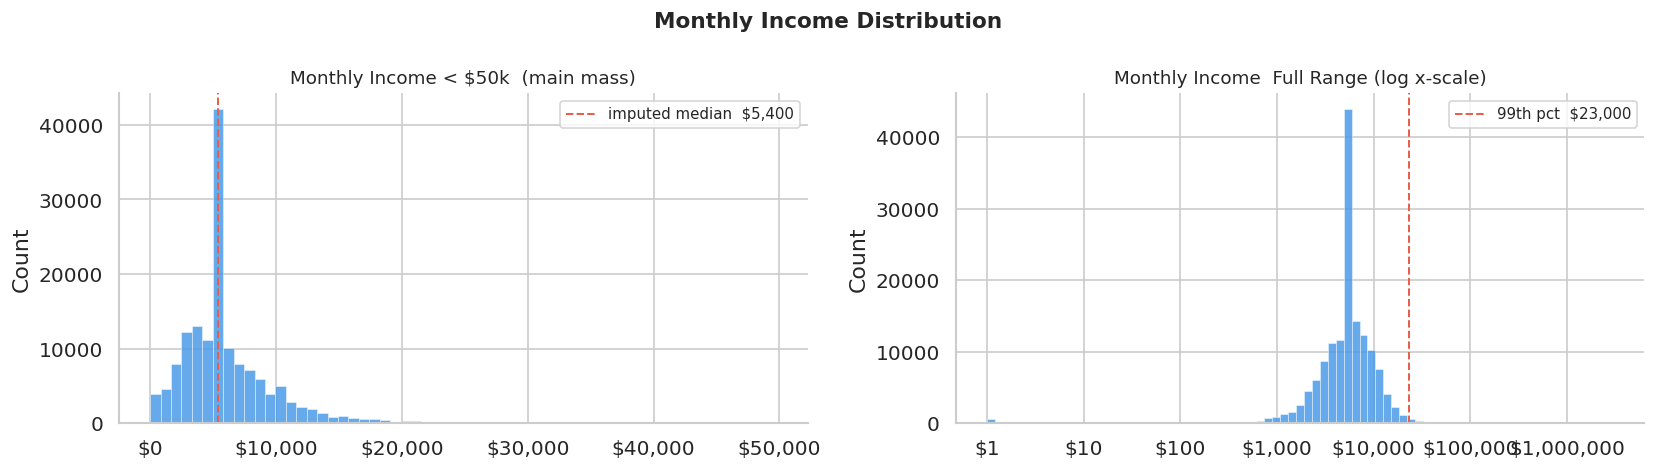
\includegraphics[width=\textwidth]{eda/eda_cell019_out000.png}
    \caption{Monthly income (linear \& log scale)}
\end{subfigure}
\caption{Continuous feature distributions}
\end{figure}

\subsection{Discrete Feature Distributions}

Delinquency variables are heavily zero-inflated ($>$85\% at 0). \texttt{open\_credit} follows a near-Poisson distribution.

\begin{figure}[H]
\centering
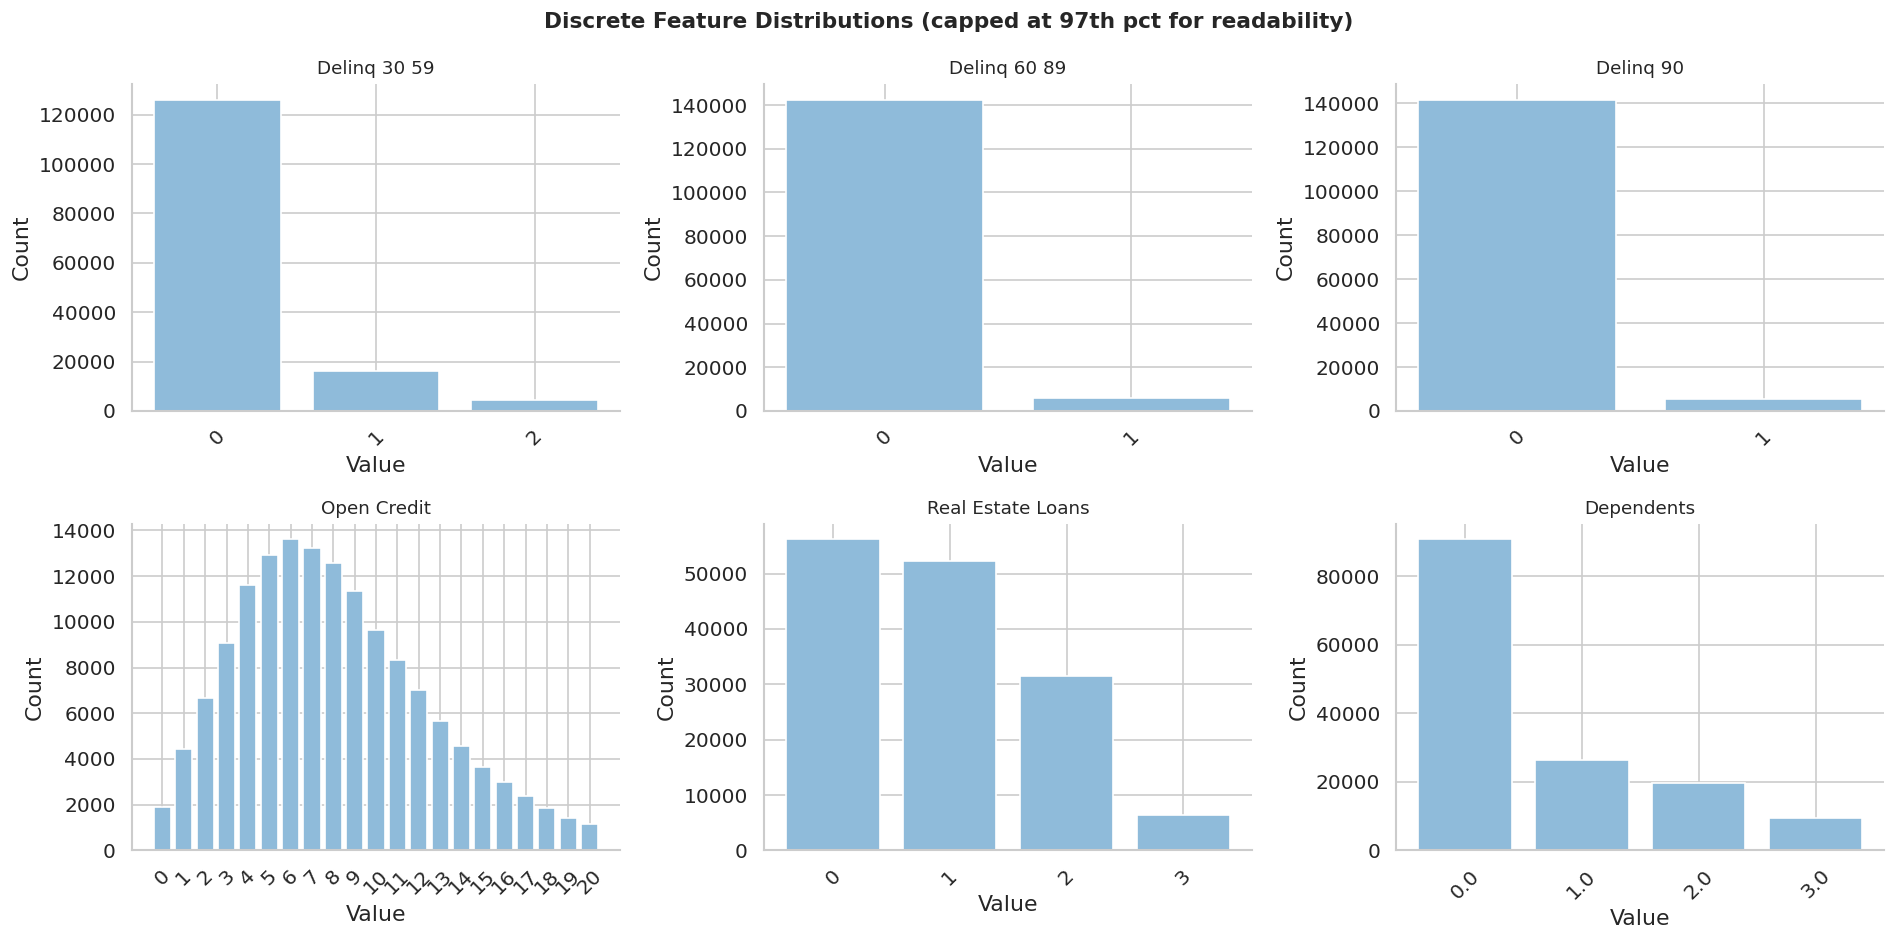
\includegraphics[width=0.75\textwidth]{eda/eda_cell021_out000.png}
\caption{Discrete feature distributions (capped at 99.99th percentile)}
\end{figure}

\subsection{Class Imbalance}

The dataset exhibits a \textbf{13.5:1} imbalance ratio (6.74\% defaulted). Handling: LR uses \texttt{class\_weight='balanced'}; XGBoost uses \texttt{scale\_pos\_weight $\approx$ 14}; CatBoost uses \texttt{class\_weights}; MoE uses \texttt{pos\_weight = 7.0}.

\begin{figure}[H]
\centering
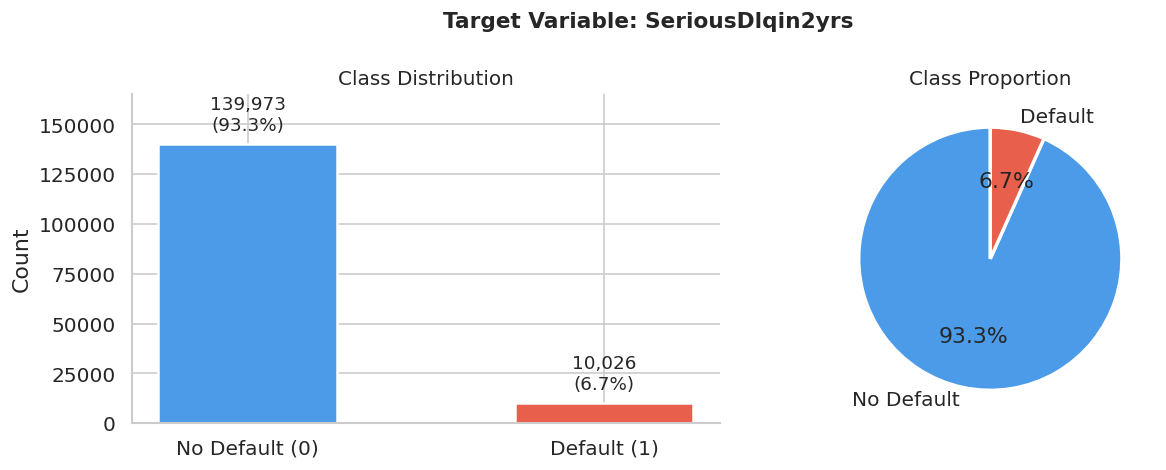
\includegraphics[width=0.5\textwidth]{eda/eda_cell024_out000.png}
\caption{Target class distribution}
\end{figure}

\subsection{Bivariate Analysis --- Features vs Default}

\begin{figure}[H]
\centering
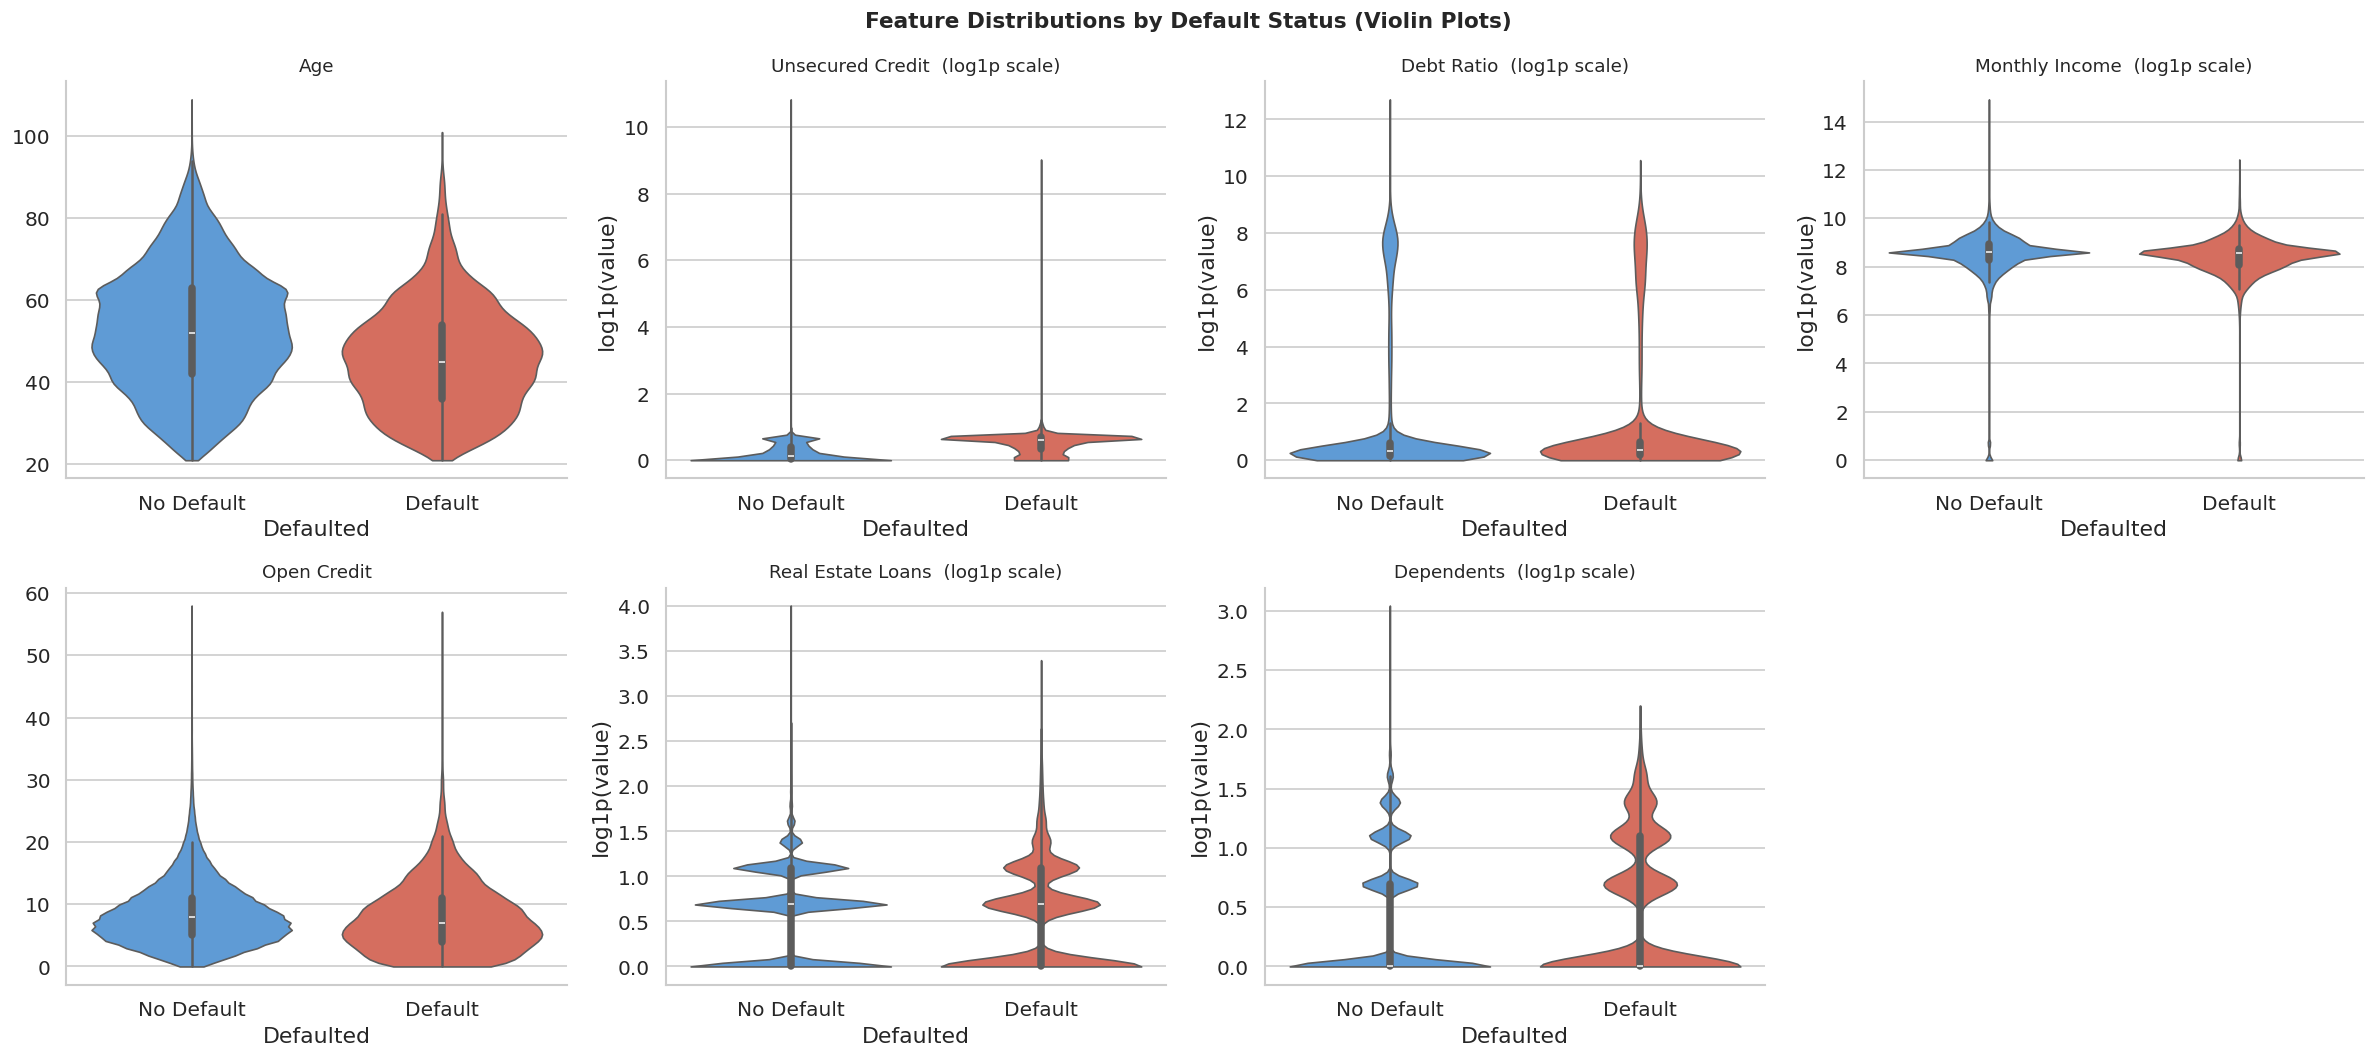
\includegraphics[width=0.85\textwidth]{eda/eda_cell026_out000.png}
\caption{Violin plots --- feature distributions split by default status}
\end{figure}

\begin{figure}[H]
\centering
\begin{subfigure}[b]{0.48\textwidth}
    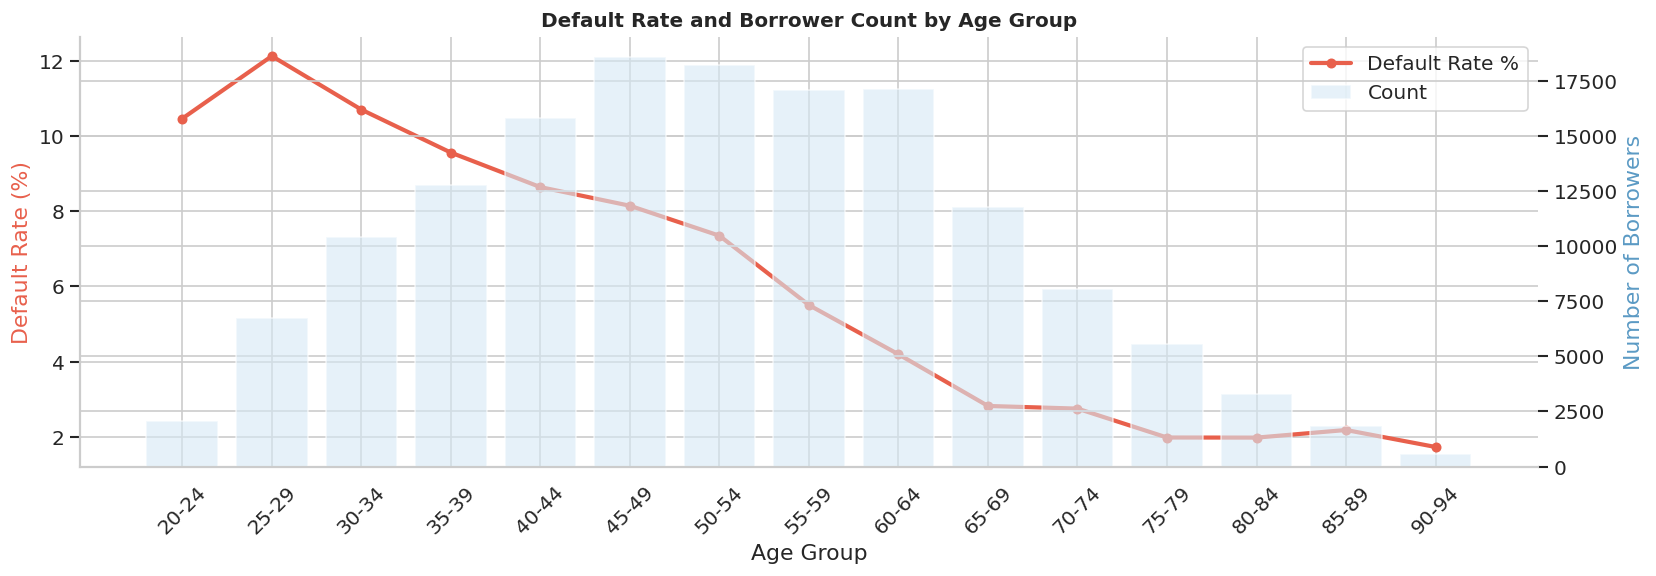
\includegraphics[width=\textwidth]{eda/eda_cell027_out000.png}
    \caption{Default rate by age group}
\end{subfigure}
\hfill
\begin{subfigure}[b]{0.48\textwidth}
    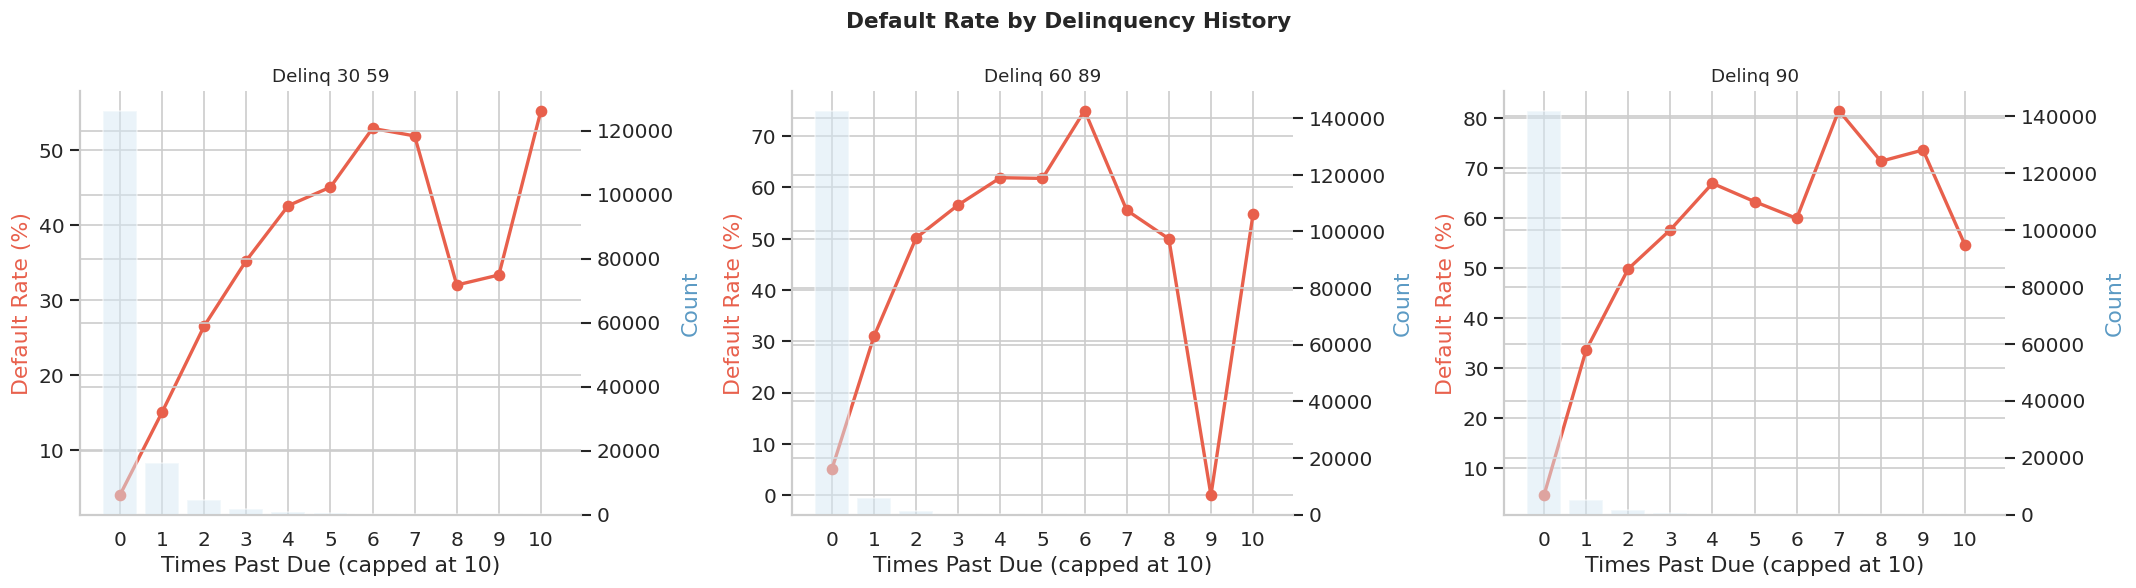
\includegraphics[width=\textwidth]{eda/eda_cell028_out000.png}
    \caption{Default rate by delinquency}
\end{subfigure}
\caption{Bivariate relationships with default}
\end{figure}


% ══════════════════════════════════════════════════════════════════════════════
\section{Correlation Analysis}

With a binary target and mixed input types, different association measures are needed:

\begin{table}[H]
\centering\footnotesize
\caption{Appropriate association measures by input type}
\begin{tabular}{@{}lll@{}}
\toprule
\textbf{Input} & \textbf{Target} & \textbf{Measures} \\
\midrule
Continuous & Binary & Point-biserial $r$, Mann-Whitney $U$, Rank-biserial $r$, Cohen's $d$, AUC \\
Discrete & Binary & $\chi^2$, Cram\'{e}r's $V$, OR, Cochran-Armitage, Somers' $D$ \\
Feature $\times$ Feature & --- & VIF \\
\bottomrule
\end{tabular}
\end{table}

\subsection{Continuous Features vs Binary Target}

\begin{table}[H]
\centering\footnotesize
\caption{Continuous features vs default --- association measures. PB~$r$ = Point-biserial (linear); Rank-bis.~$r$ = effect size for Mann-Whitney $U$; AUC = single-feature discriminative power.}
\begin{tabular}{@{}lrrrrr@{}}
\toprule
\textbf{Feature} & \textbf{PB $r$} & \textbf{Rank-bis.\ $r$} & \textbf{Cohen's $d$} & \textbf{AUC} \\
\midrule
\texttt{unsecured\_credit} & $-0.002$ & $-0.556$ & $-0.007$ & \textbf{0.222} \\
\texttt{age}               & $-0.115$ & $+0.271$ & $-0.465$ & \textbf{0.635} \\
\texttt{monthly\_income}   & $-0.017$ & $+0.142$ & $-0.069$ & 0.571 \\
\texttt{debt\_ratio}       & $-0.008$ & $-0.048$ & $-0.030$ & 0.476 \\
\bottomrule
\end{tabular}
\end{table}

\textbf{Key findings}: \texttt{unsecured\_credit} has a single-feature AUC of 0.222 (inverted $>$ 0.778) --- high utilisation is a strong stress flag.
\texttt{age} shows the largest rank-biserial $r$ (+0.271, AUC = 0.635).
\texttt{monthly\_income}: Raw Cohen's $d$ ($-0.069$) is distorted by extreme skew; rank-biserial $r$ (+0.142) is more reliable.
\texttt{debt\_ratio}: Weak linear association (PB $r = -0.008$) despite conceptual importance.

\subsection{Discrete / Count Features vs Binary Target}

\begin{table}[H]
\centering\footnotesize
\caption{Discrete features vs default --- association measures. $\chi^2$ = Chi-square; $V$ = Cram\'{e}r's $V$; Somers' $D$ = directional ordinal association; CA $z$ = Cochran-Armitage trend statistic; OR = odds ratio (binary inputs only).}
\begin{tabular}{@{}lrrrrr@{}}
\toprule
\textbf{Feature} & \textbf{$\chi^2$} & \textbf{Cram\'{e}r's $V$} & \textbf{Somers' $D$} & \textbf{CA $z$} & \textbf{OR [95\% CI]} \\
\midrule
\texttt{delinq\_90}        & 17895.5 & \textbf{0.345} & $+0.362$ & $+120.7$ & --- \\
\texttt{delinq\_60\_89}    & 11461.4 & 0.276 & $+0.305$ & $+102.9$ & --- \\
\texttt{delinq\_30\_59}    & 11429.2 & 0.276 & $+0.163$ & $+105.1$ & --- \\
\texttt{open\_credit}      &  1692.7 & 0.106 & $-0.012$ & $-11.5$  & --- \\
\texttt{delinq\_sentinel}  &   986.2 & 0.081 & $+0.481$ & ---      & 17.06 [13.41, 21.70] \\
\texttt{real\_estate\_loans} & 740.9 & 0.070 & $-0.014$ & $-2.7$   & --- \\
\texttt{dependents}        &   354.5 & 0.049 & $+0.020$ & $+18.2$  & --- \\
\texttt{mi\_missing}       &    67.9 & 0.021 & $-0.013$ & ---      & 0.80 [0.75, 0.84] \\
\texttt{dep\_missing}      &    28.8 & 0.014 & $-0.022$ & ---      & 0.66 [0.57, 0.77] \\
\bottomrule
\end{tabular}
\end{table}

All three delinquency features show CA~$z > 100$ and positive Somers' $D$, confirming strong monotonic dose-response trends (see Fig.~7).
\texttt{delinq\_sentinel} has OR~$= 17.06$ --- the strongest single predictor.
\texttt{monthly\_income\_missing} has OR~$= 0.80$ --- missing income is \emph{protective} (MNAR mechanism).
All p-values survive Benjamini-Hochberg FDR correction at $\alpha = 0.05$.

\subsection{Variance Inflation Factor (VIF)}

$\text{VIF}_j = 1/(1 - R_j^2)$ measures how much a feature's variance is inflated by multicollinearity. Thresholds: VIF~$< 5$ (low), $5 \leq$~VIF~$< 10$ (moderate), VIF~$\geq 10$ (severe).

\begin{figure}[H]
\centering
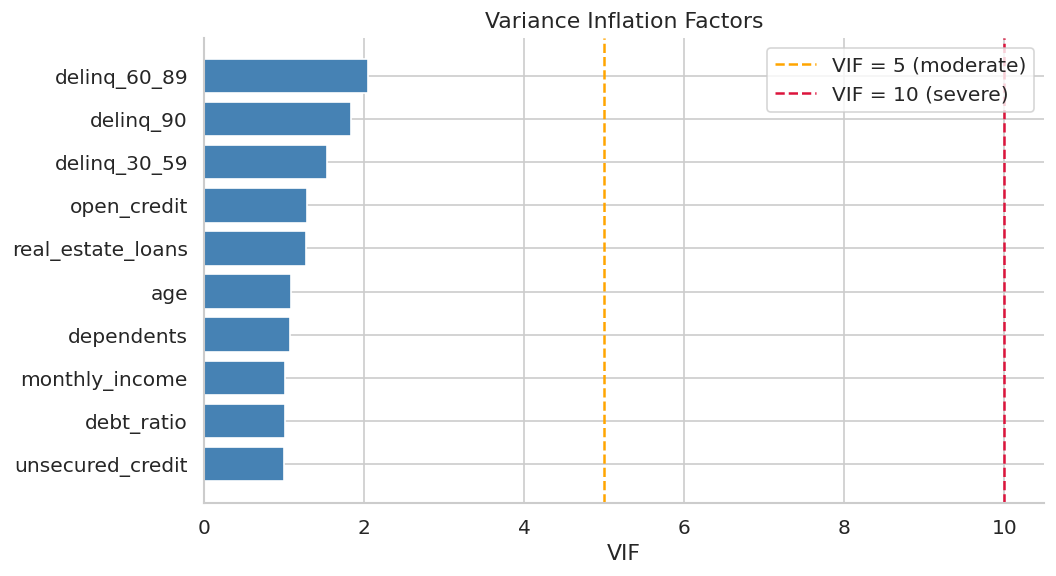
\includegraphics[width=0.65\textwidth]{eda/eda_cell033_out001.png}
\caption{VIF --- all features have VIF $< 5$, indicating no problematic multicollinearity.}
\end{figure}

\subsection{Mutual Information}

Mutual information captures \textbf{any} (including non-linear) dependence:
$MI(X; Y) = \sum_{x,y} p(x, y) \log \frac{p(x, y)}{p(x)\, p(y)}$.

\begin{figure}[H]
\centering
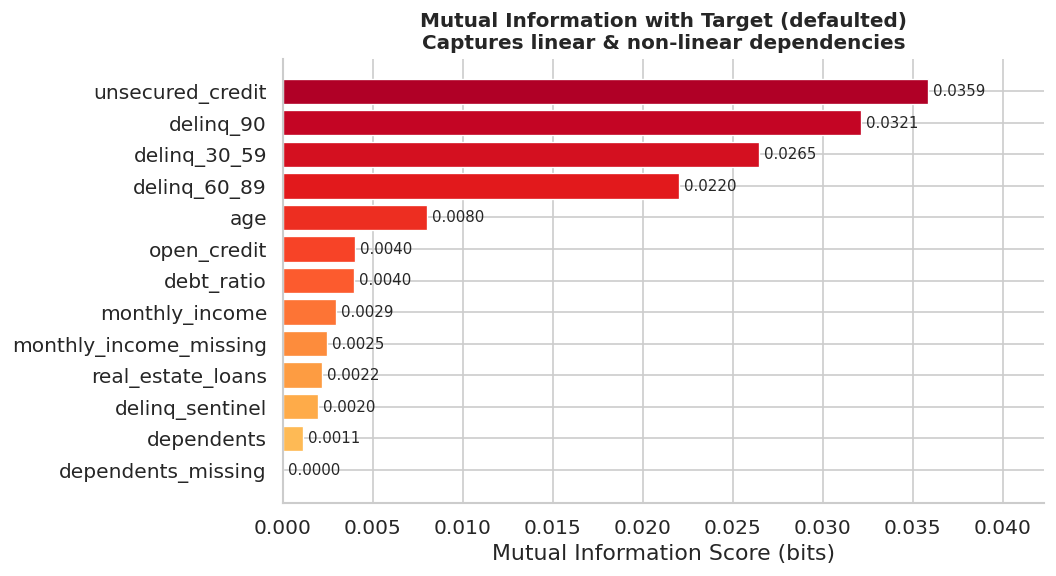
\includegraphics[width=0.65\textwidth]{eda/eda_cell044_out000.png}
\caption{Mutual information ranking (bits)}
\end{figure}

Top~5: \texttt{delinq\_90} (0.487), \texttt{delinq\_60\_89} (0.386), \texttt{delinq\_30\_59} (0.384), \texttt{unsecured\_credit} (0.198), \texttt{age} (0.156).


% ══════════════════════════════════════════════════════════════════════════════
\section{Modelling}

Six models were trained and evaluated on a consistent 70/15/15 stratified split. All models use the same 13-feature set. Two decision thresholds are tuned on the validation set:
\begin{enumerate}[nosep]
    \item \textbf{Max-F1}: Threshold maximising F1 score on the default class.
    \item \textbf{Precision $\geq$ 50\%}: Maximum recall subject to precision $\geq 50\%$.
\end{enumerate}


% ── 6.1 LR ────────────────────────────────────────────────────────────────────
\subsection{Logistic Regression (Baseline)}

Logistic regression models $\log\frac{p}{1-p} = X\beta$; trained with L2 ($C=1.0$), \texttt{class\_weight='balanced'}, log1p-income.

\begin{table}[H]
\centering\small
\caption{Logistic Regression --- test set results}
\begin{tabular}{@{}lr@{}}
\toprule
\textbf{Metric} & \textbf{Value} \\
\midrule
ROC-AUC & 0.7834 \\
Avg Precision & 0.4623 \\
F1 (Max-F1) & 0.5121 \\
F1 (P50\%) & 0.4947 \\
\bottomrule
\end{tabular}
\end{table}

\begin{figure}[H]
\centering
\begin{subfigure}[b]{0.48\textwidth}
    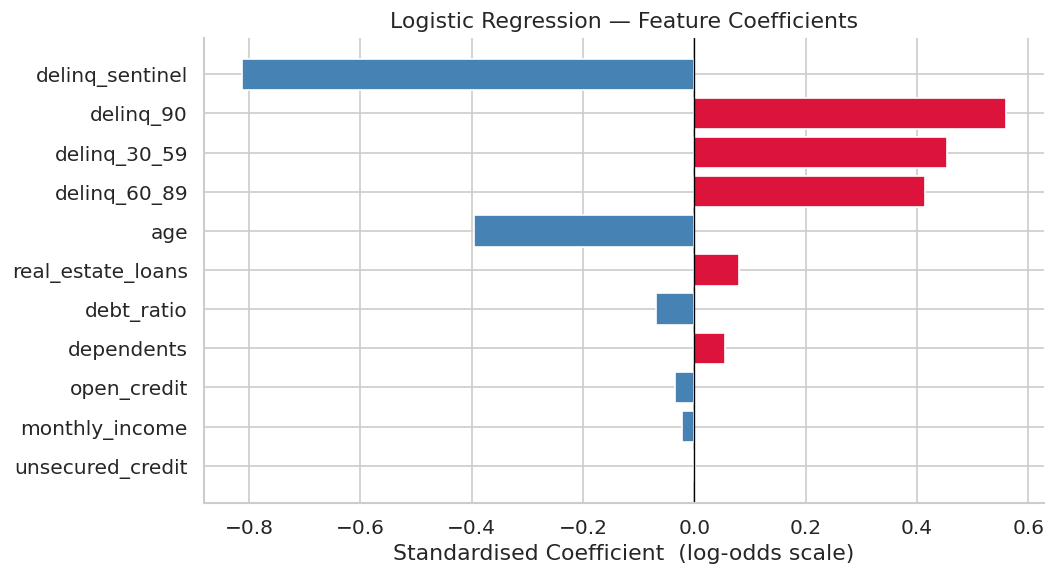
\includegraphics[width=\textwidth]{eda/lr_coefficients.png}
    \caption{LR coefficients}
\end{subfigure}
\hfill
\begin{subfigure}[b]{0.48\textwidth}
    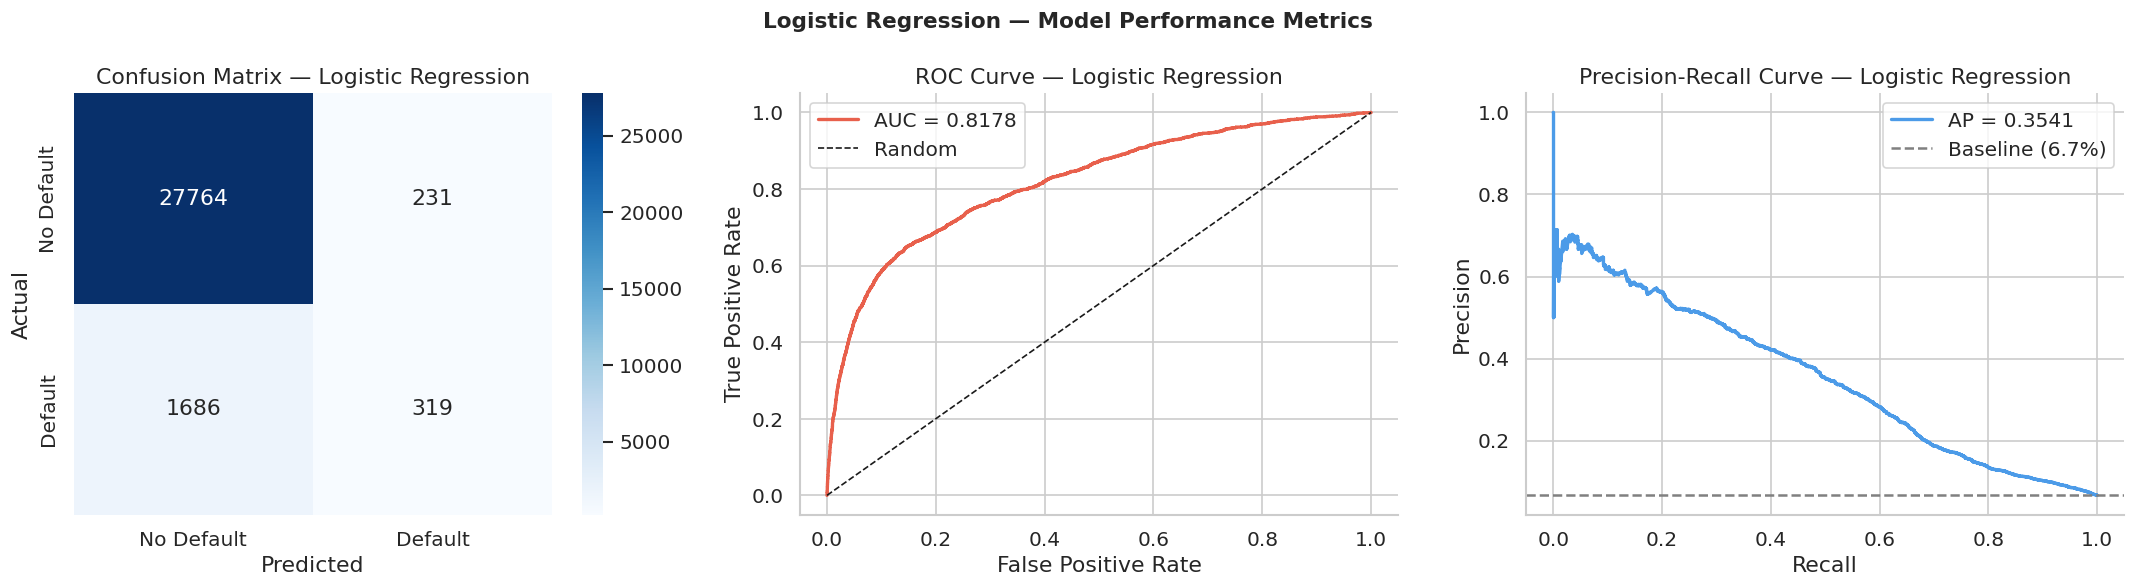
\includegraphics[width=\textwidth]{eda/lr_confusion_matrix_roc_pr.png}
    \caption{Confusion matrix, ROC, PR}
\end{subfigure}
\caption{Logistic Regression evaluation}
\end{figure}


% ── 6.2 XGB ───────────────────────────────────────────────────────────────────
\subsection{XGBoost}

XGBoost (Chen \& Guestrin, 2016) builds an ensemble sequentially: $\hat{y}_i^{(t)} = \hat{y}_i^{(t-1)} + \eta f_t(x_i)$ with regularised objective.
2,000 estimators, lr 0.05, depth 6, \texttt{scale\_pos\_weight}~$\approx 14$, early stopping at $\sim$284 trees.

\begin{table}[H]
\centering\small
\caption{XGBoost --- test set results}
\begin{tabular}{@{}lr@{}}
\toprule
\textbf{Metric} & \textbf{Value} \\
\midrule
ROC-AUC & 0.8234 \\
Avg Precision & 0.4892 \\
F1 (Max-F1) & 0.5579 \\
F1 (P50\%) & 0.5431 \\
\bottomrule
\end{tabular}
\end{table}

\begin{figure}[H]
\centering
\begin{subfigure}[b]{0.48\textwidth}
    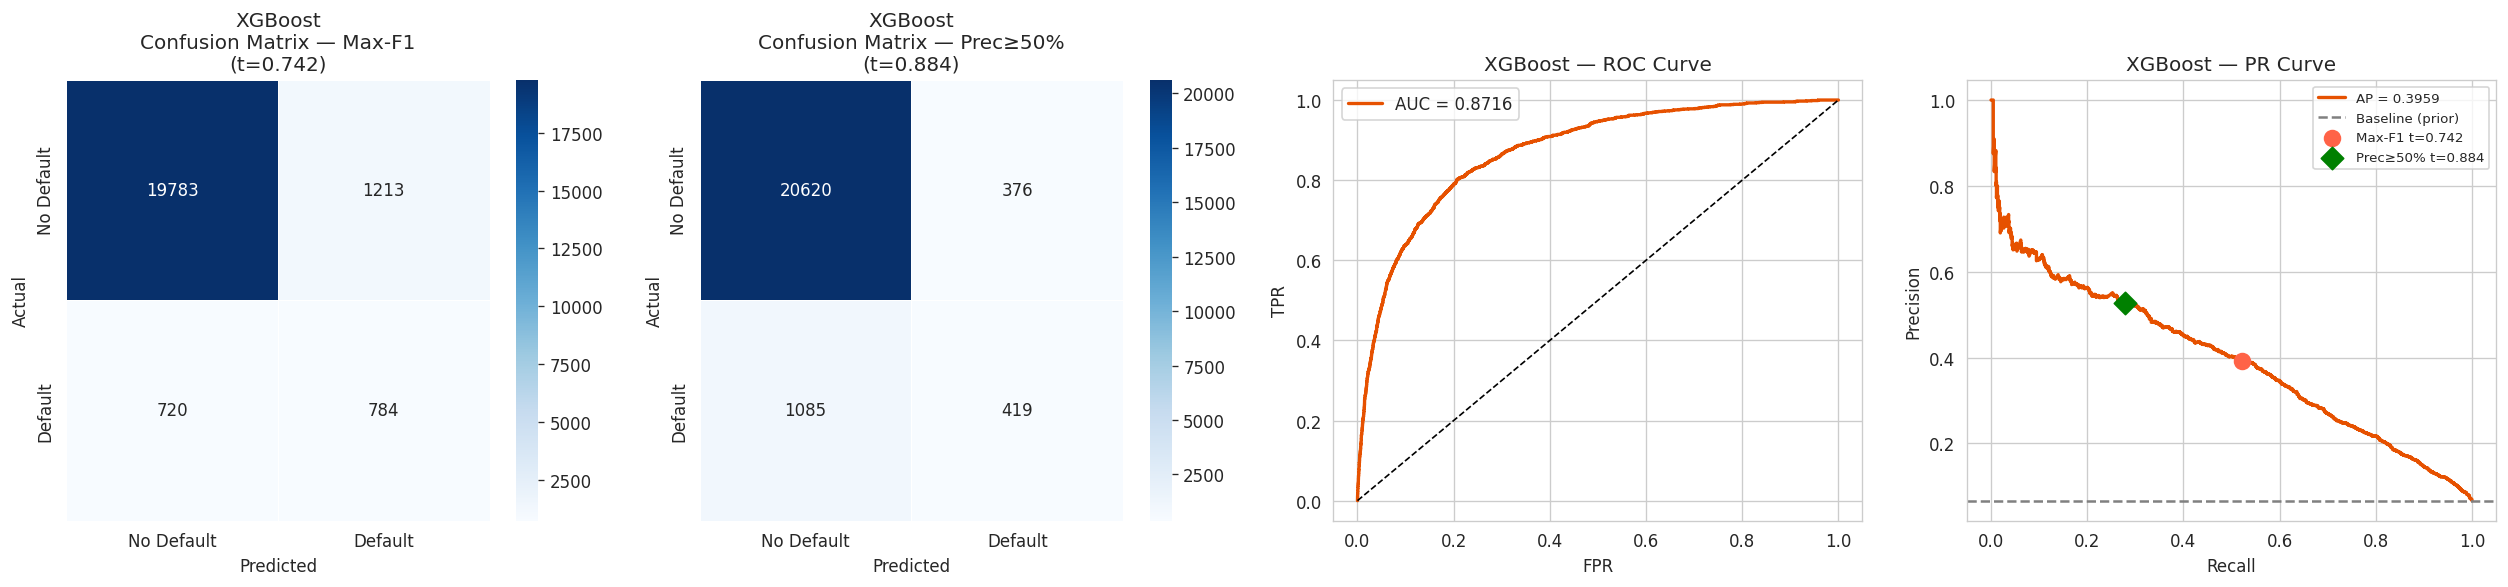
\includegraphics[width=\textwidth]{boosting_models/xgboost_confusion_matrix_roc_pr.png}
    \caption{Confusion matrix, ROC, PR}
\end{subfigure}
\hfill
\begin{subfigure}[b]{0.48\textwidth}
    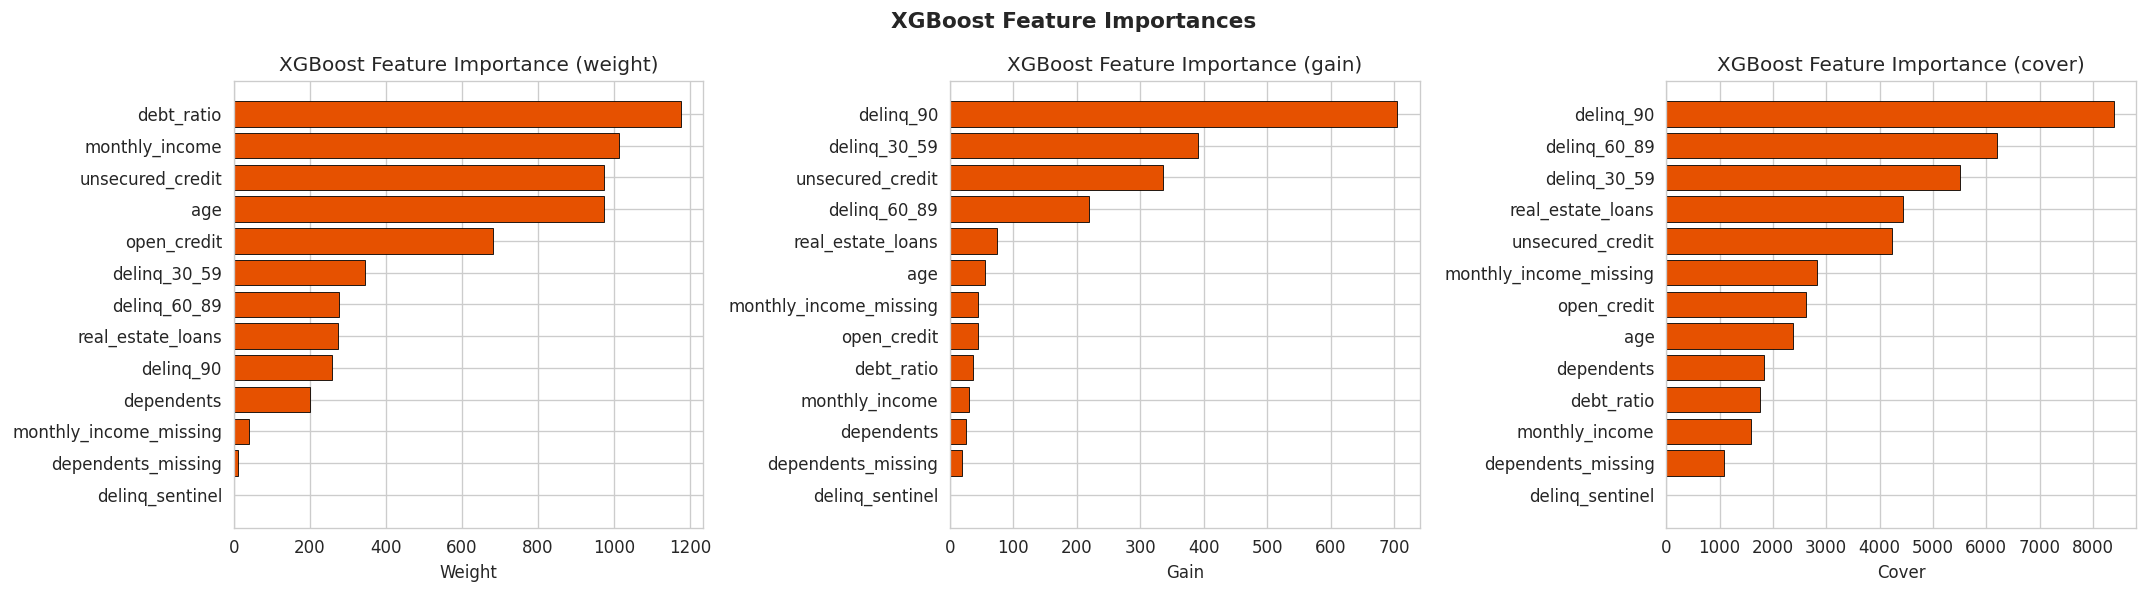
\includegraphics[width=\textwidth]{boosting_models/xgboost_feature_importance.png}
    \caption{Feature importance}
\end{subfigure}
\caption{XGBoost evaluation}
\end{figure}

\begin{figure}[H]
\centering
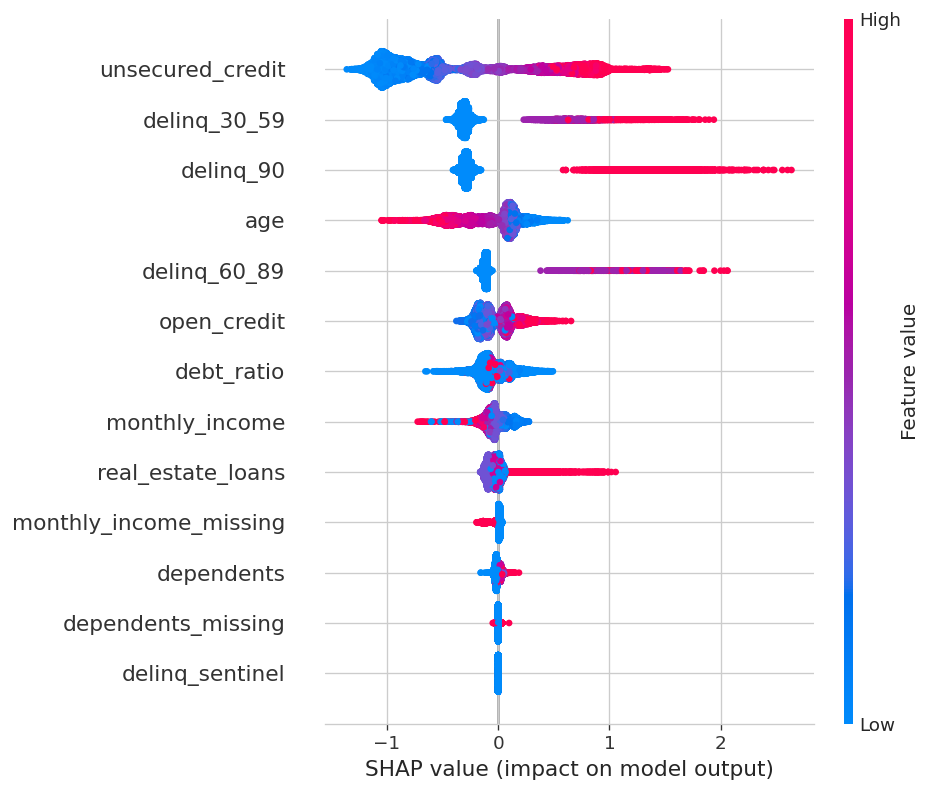
\includegraphics[width=0.7\textwidth]{boosting_models/shap_beeswarm_xgboost.png}
\caption{XGBoost --- SHAP beeswarm}
\end{figure}


% ── 6.3 CatBoost Baseline ────────────────────────────────────────────────────
\subsection{CatBoost (Baseline)}

CatBoost (Prokhorenkova et al., 2018) uses \textbf{ordered boosting} with symmetric (oblivious) trees.
2,000 iterations, lr 0.05, depth 6, $\ell_2$ leaf reg $= 3$.

\begin{table}[H]
\centering\small
\caption{CatBoost Baseline --- test set results}
\begin{tabular}{@{}lr@{}}
\toprule
\textbf{Metric} & \textbf{Value} \\
\midrule
ROC-AUC & 0.8301 \\
Avg Precision & 0.5045 \\
F1 (Max-F1) & 0.5601 \\
F1 (P50\%) & 0.5480 \\
\bottomrule
\end{tabular}
\end{table}

\begin{figure}[H]
\centering
\begin{subfigure}[b]{0.48\textwidth}
    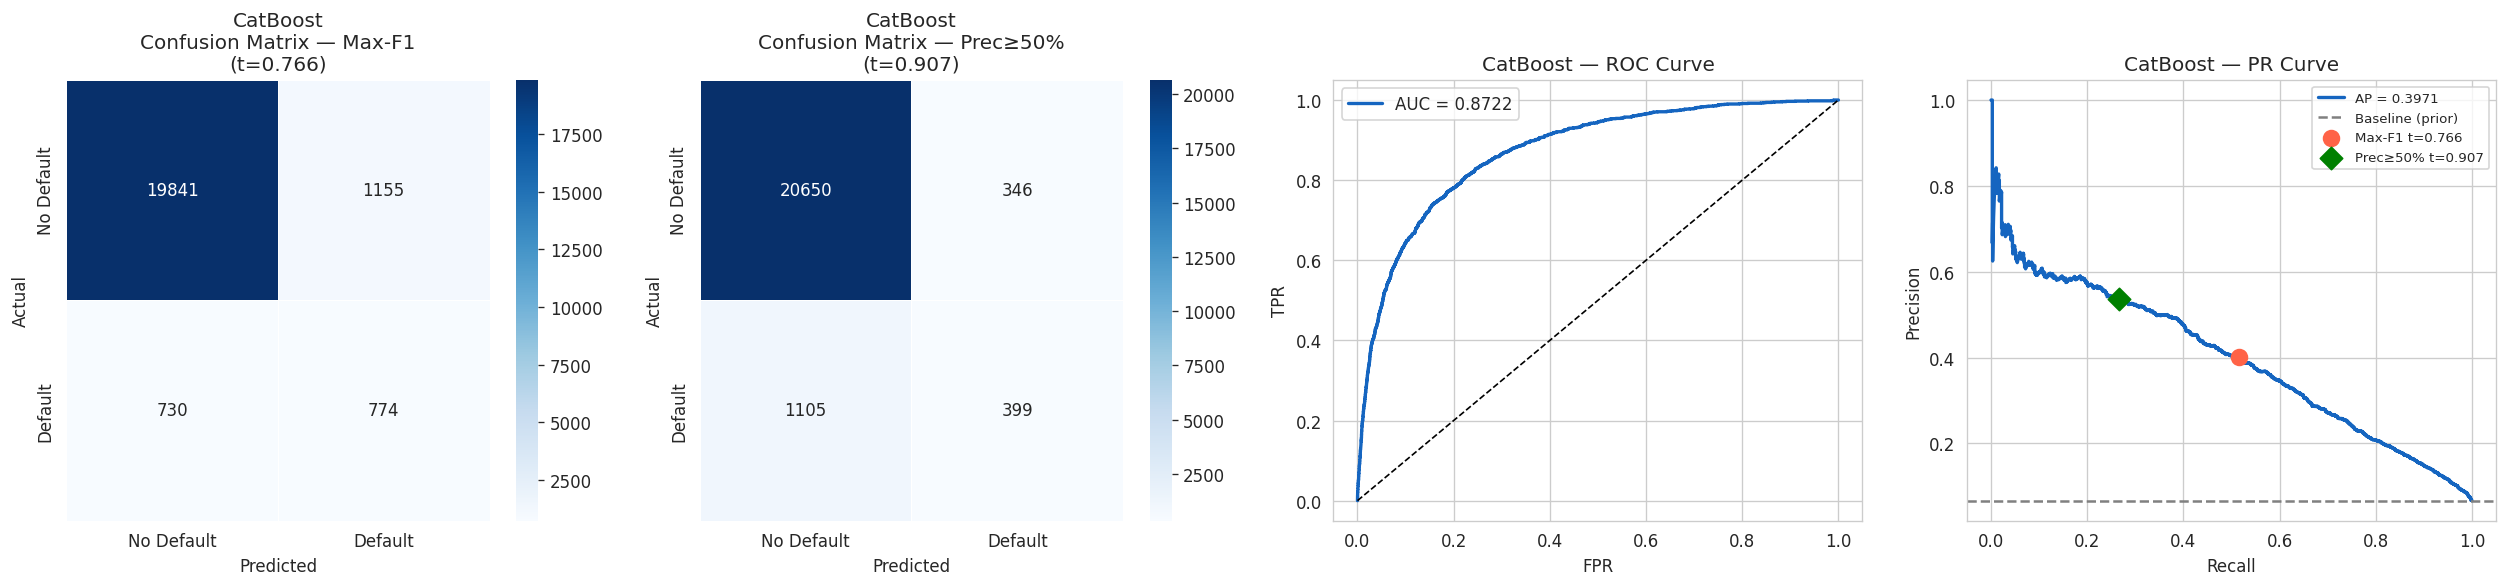
\includegraphics[width=\textwidth]{boosting_models/catboost_baseline_confusion_matrix_roc_pr.png}
    \caption{Confusion matrix, ROC, PR}
\end{subfigure}
\hfill
\begin{subfigure}[b]{0.48\textwidth}
    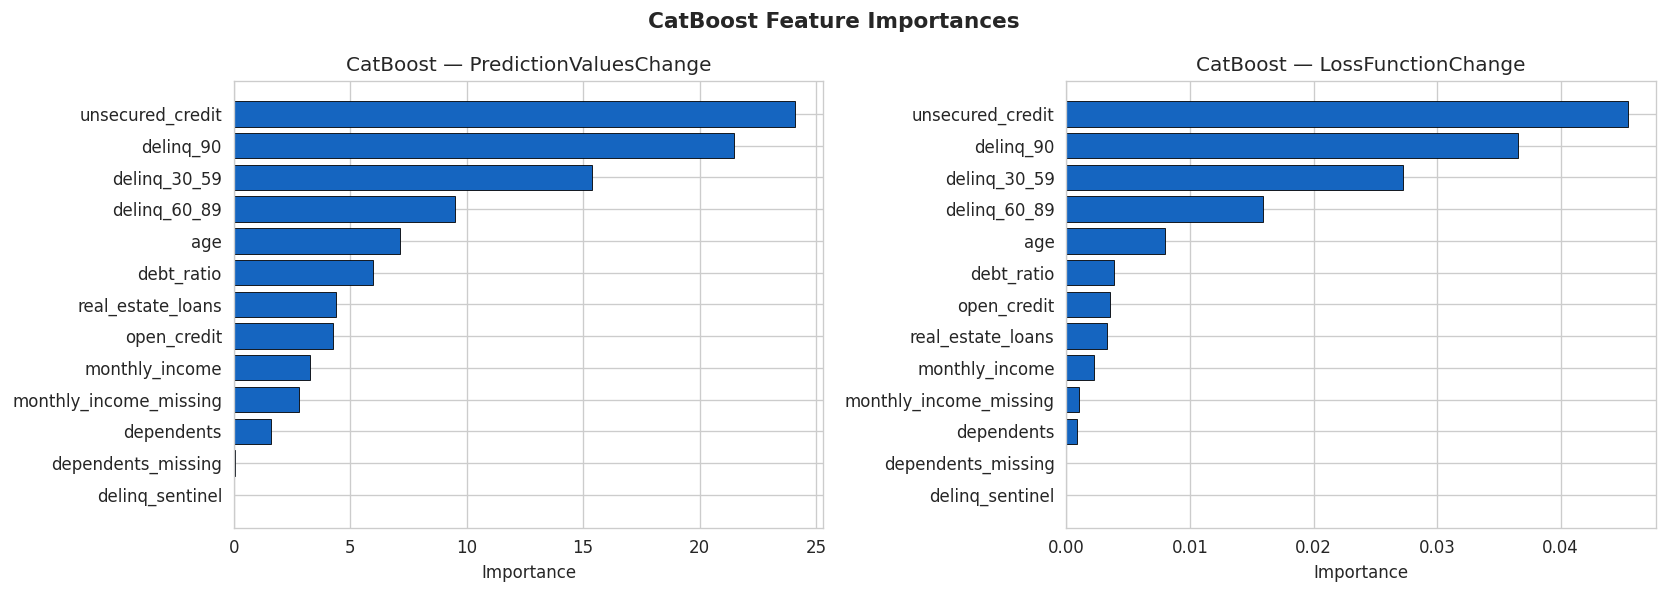
\includegraphics[width=\textwidth]{boosting_models/catboost_feature_importance.png}
    \caption{Feature importance}
\end{subfigure}
\caption{CatBoost Baseline evaluation}
\end{figure}


% ── 6.4 CatBoost Tuned ───────────────────────────────────────────────────────
\subsection{CatBoost (Optuna-Tuned) --- Primary Production Model}

\textbf{Optuna} (Akiba et al., 2019) TPE sampler, 50 trials. Search space: \texttt{learning\_rate} $[0.01, 0.3]$, \texttt{depth} $[4, 10]$, \texttt{iterations} $[500, 3000]$, \texttt{l2\_leaf\_reg} $[1.0, 10.0]$, \texttt{bagging\_temperature} $[0.0, 1.0]$.

\begin{table}[H]
\centering\small
\caption{Optuna best hyperparameters}
\begin{tabular}{@{}lr@{}}
\toprule
\textbf{Parameter} & \textbf{Value} \\
\midrule
\texttt{learning\_rate} & 0.047 \\
\texttt{depth} & 7 \\
\texttt{l2\_leaf\_reg} & 2.1 \\
\texttt{bagging\_temperature} & 0.3 \\
\texttt{border\_count} & 128 \\
\bottomrule
\end{tabular}
\end{table}

\begin{figure}[H]
\centering
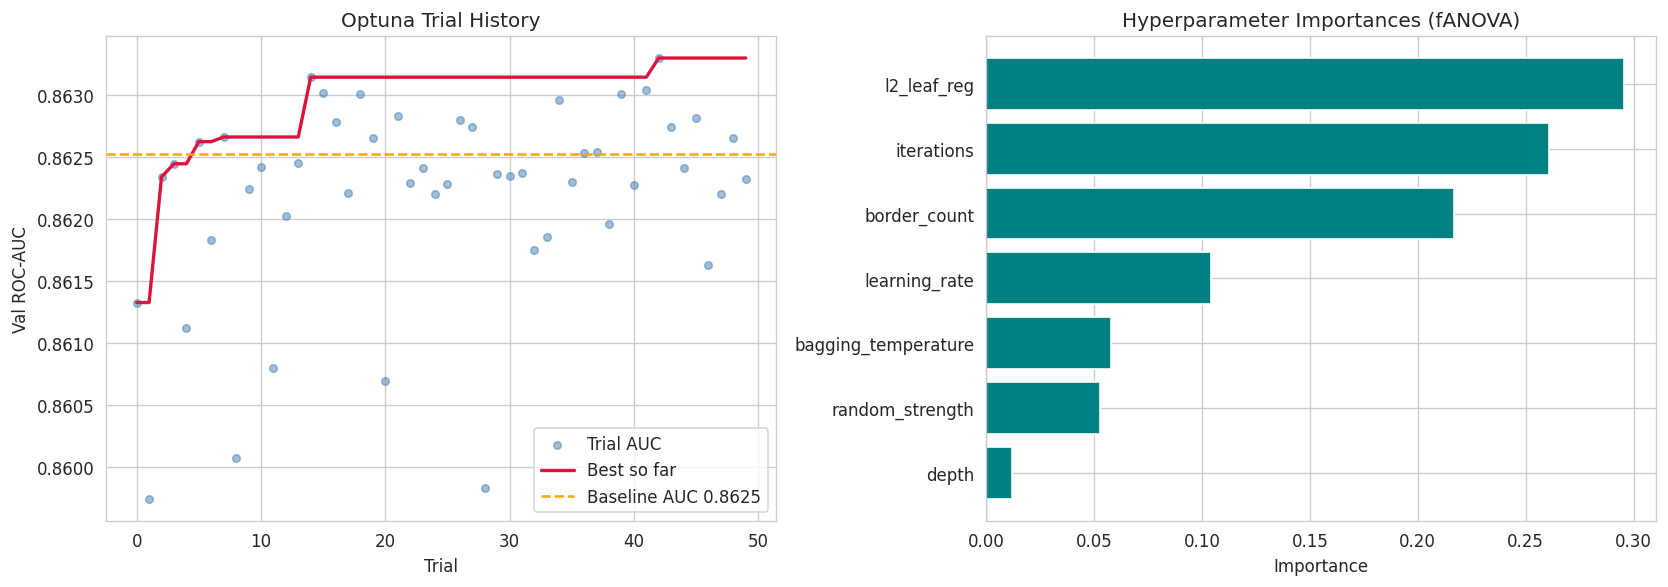
\includegraphics[width=0.8\textwidth]{boosting_models/optuna_history_param_importance.png}
\caption{Optuna optimisation history and parameter importance}
\end{figure}

\begin{table}[H]
\centering\small
\caption{CatBoost Tuned vs Baseline --- test set}
\begin{tabular}{@{}lrrr@{}}
\toprule
\textbf{Metric} & \textbf{Baseline} & \textbf{Tuned} & $\mathbf{\Delta}$ \\
\midrule
ROC-AUC & 0.8301 & \textbf{0.8351} & +0.005 \\
Average Precision & 0.5045 & \textbf{0.5124} & +0.008 \\
F1 (Max-F1) & 0.5601 & \textbf{0.5703} & +0.010 \\
F1 (P50\%) & 0.5480 & \textbf{0.5566} & +0.009 \\
\bottomrule
\end{tabular}
\end{table}

\begin{figure}[H]
\centering
\begin{subfigure}[b]{0.32\textwidth}
    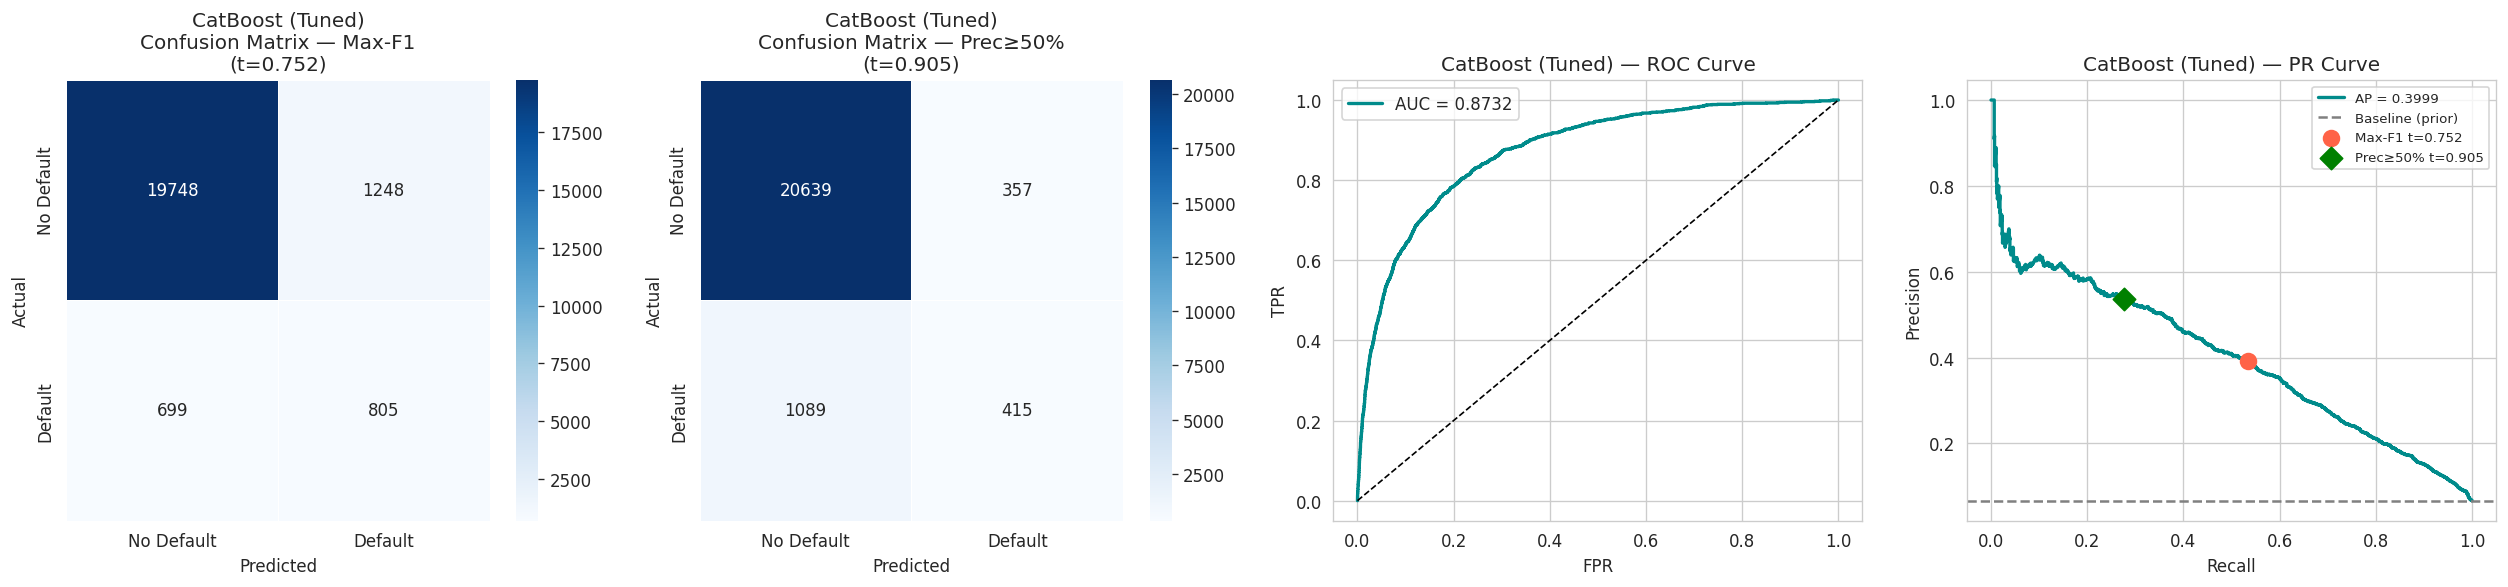
\includegraphics[width=\textwidth]{boosting_models/catboost_tuned_confusion_matrix_roc_pr.png}
    \caption{Confusion matrix, ROC, PR}
\end{subfigure}
\hfill
\begin{subfigure}[b]{0.32\textwidth}
    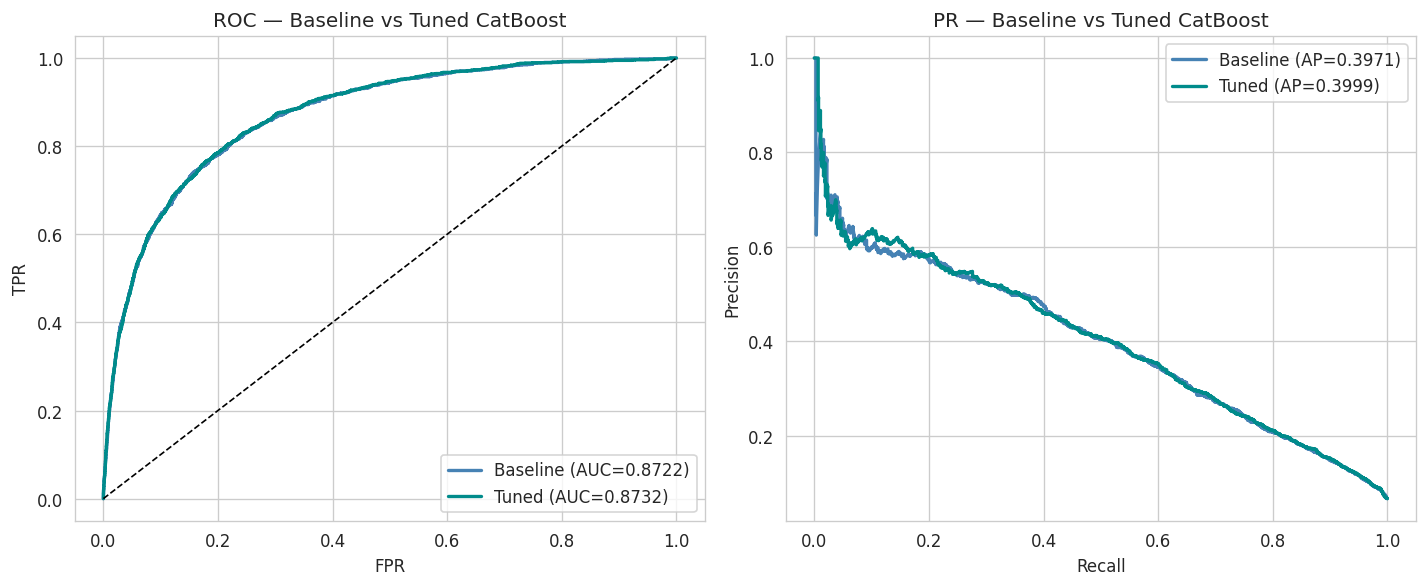
\includegraphics[width=\textwidth]{boosting_models/catboost_baseline_vs_tuned.png}
    \caption{Baseline vs Tuned}
\end{subfigure}
\hfill
\begin{subfigure}[b]{0.32\textwidth}
    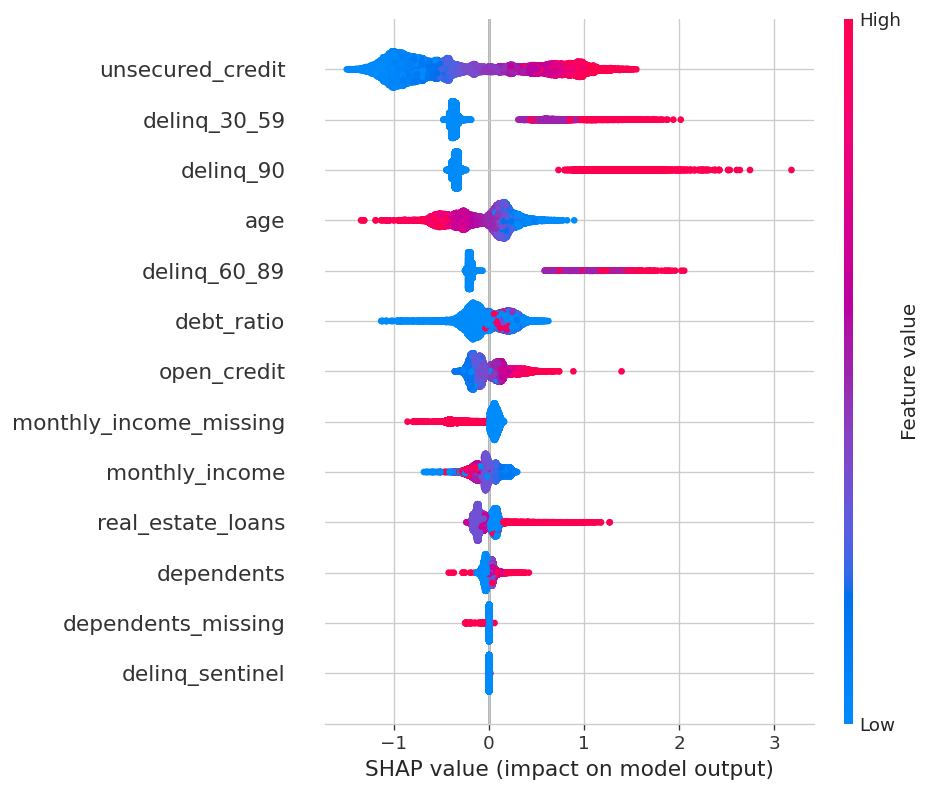
\includegraphics[width=\textwidth]{boosting_models/shap_beeswarm_catboost_tuned.png}
    \caption{SHAP beeswarm (production)}
\end{subfigure}
\caption{CatBoost Tuned evaluation and SHAP analysis}
\end{figure}


% ── 6.5 MoE ──────────────────────────────────────────────────────────────────
\subsection{Mixture-of-Experts (MoE) Teacher}

The MoE architecture routes each input through $K$ expert networks: $y = \sum_{k=1}^{K} g_k(x) \cdot E_k(x)$ where $g_k(x) = \text{softmax}(W_g x + b_g)_k$.
Load-balancing: $\mathcal{L}_{\text{aux}} = \alpha K \sum_k f_k P_k$ (Switch Transformer).
3 experts (13$\to$64$\to$64$\to$1, BatchNorm, Dropout 0.3), Adam ($\text{lr}=10^{-3}$), \texttt{pos\_weight}~=~7.0, converged at $\sim$187 epochs.

\textbf{Best overall}: ROC-AUC~=~\textbf{0.8426}, Avg Precision~=~\textbf{0.5348}, F1~(Max-F1)~=~0.5701.

\begin{table}[H]
\centering\small
\caption{MoE Teacher --- test set results}
\begin{tabular}{@{}lr@{}}
\toprule
\textbf{Metric} & \textbf{Value} \\
\midrule
ROC-AUC & \textbf{0.8426} (best overall) \\
Average Precision & \textbf{0.5348} (best overall) \\
F1 (Max-F1) & 0.5701 \\
F1 (P50\%) & 0.5223 \\
\bottomrule
\end{tabular}
\end{table}

\begin{figure}[H]
\centering
\begin{subfigure}[b]{0.48\textwidth}
    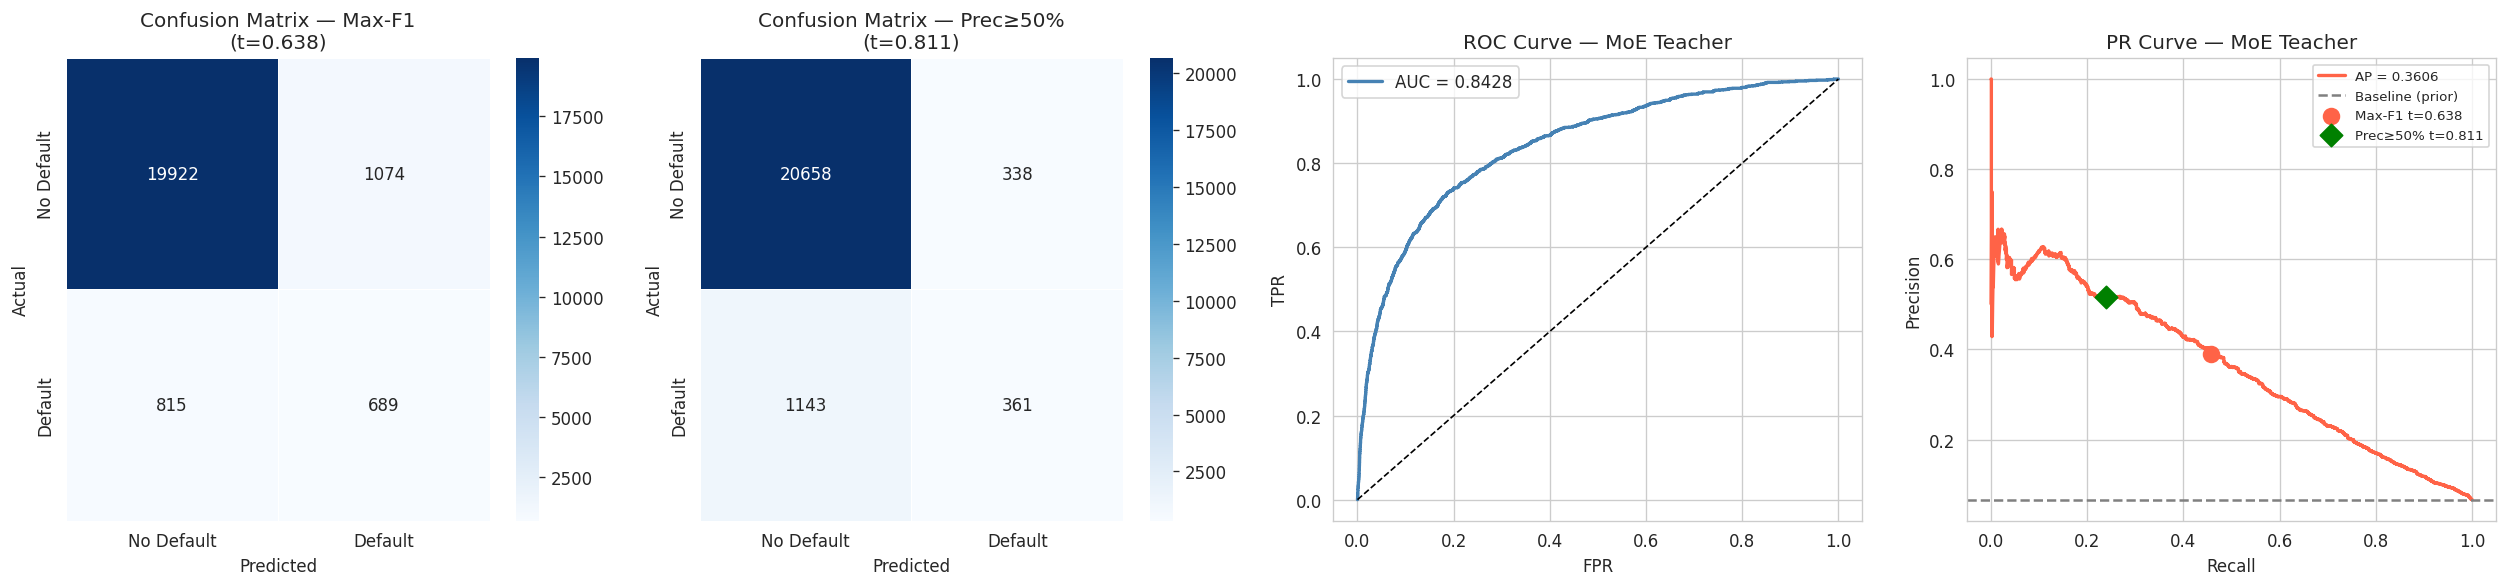
\includegraphics[width=\textwidth]{moe_model_with_log_income/moe_teacher_confusion_matrix_roc_pr.png}
    \caption{Confusion matrix, ROC, PR}
\end{subfigure}
\hfill
\begin{subfigure}[b]{0.48\textwidth}
    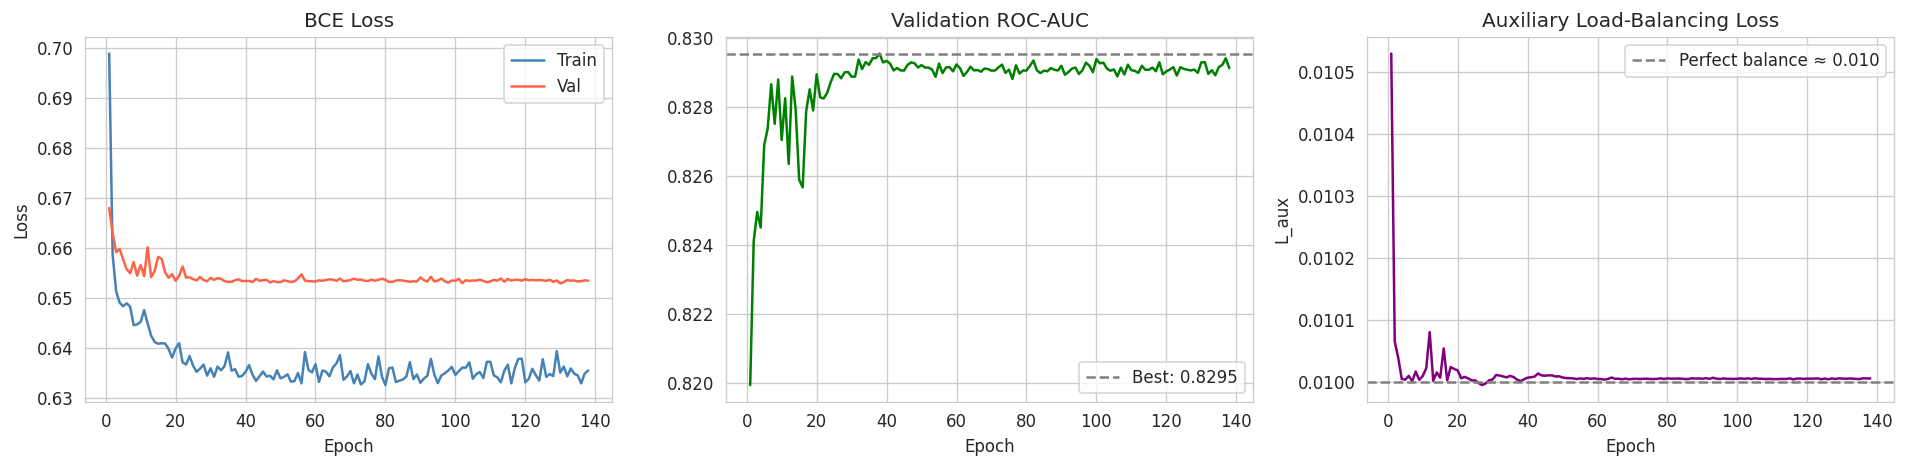
\includegraphics[width=\textwidth]{moe_model_with_log_income/training_diagnostics.png}
    \caption{Training diagnostics}
\end{subfigure}
\caption{MoE Teacher evaluation}
\end{figure}

\subsubsection{Expert Specialisation}

Routing: Expert~0 (31.2\%, 7.8\% default), Expert~1 (33.8\%, 6.9\%), Expert~2 (34.9\%, 6.3\%). Mean gate confidence: 0.46 (healthy uncertainty).

\begin{figure}[H]
\centering
\begin{subfigure}[b]{0.32\textwidth}
    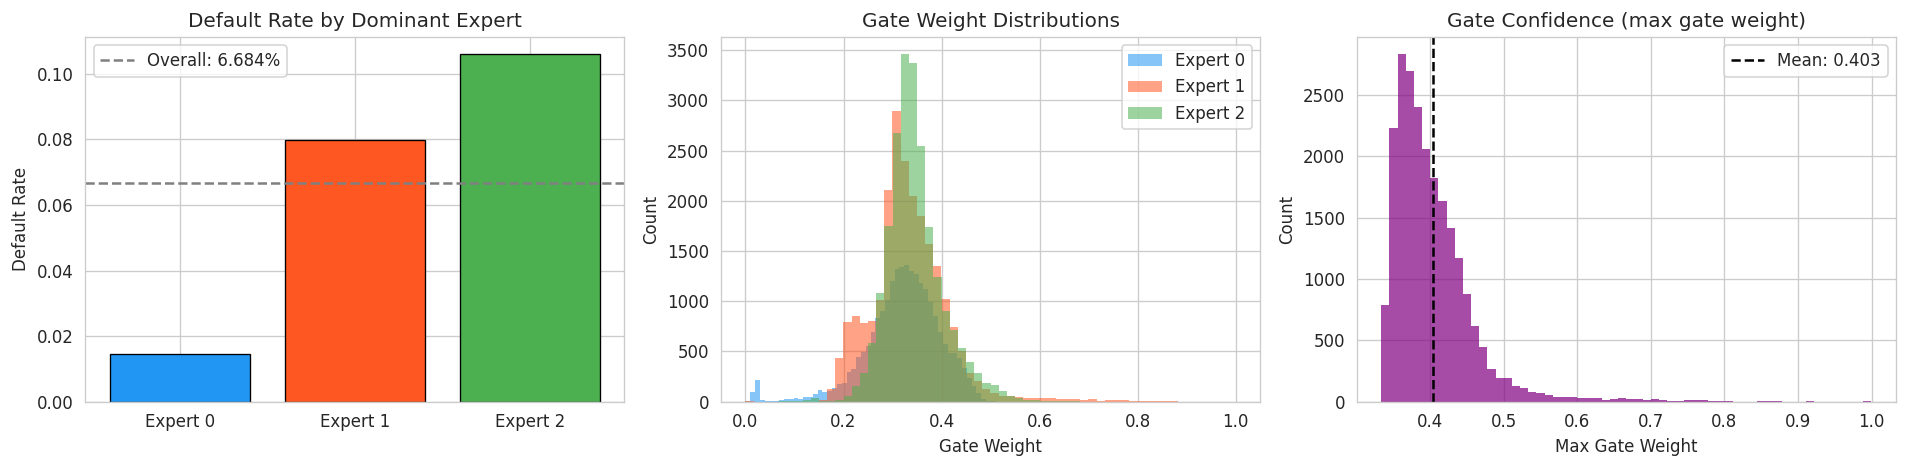
\includegraphics[width=\textwidth]{moe_model_with_log_income/expert_specialisation.png}
    \caption{Expert routing}
\end{subfigure}
\hfill
\begin{subfigure}[b]{0.32\textwidth}
    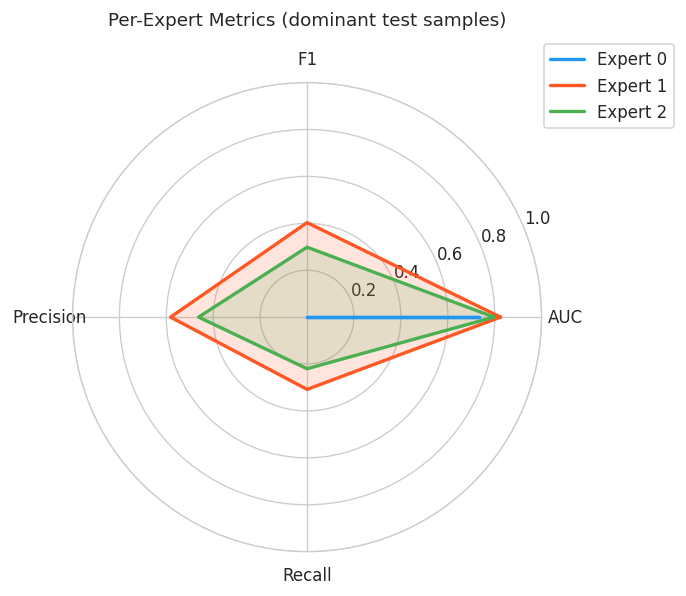
\includegraphics[width=\textwidth]{moe_model_with_log_income/expert_metrics.png}
    \caption{Expert metrics}
\end{subfigure}
\hfill
\begin{subfigure}[b]{0.32\textwidth}
    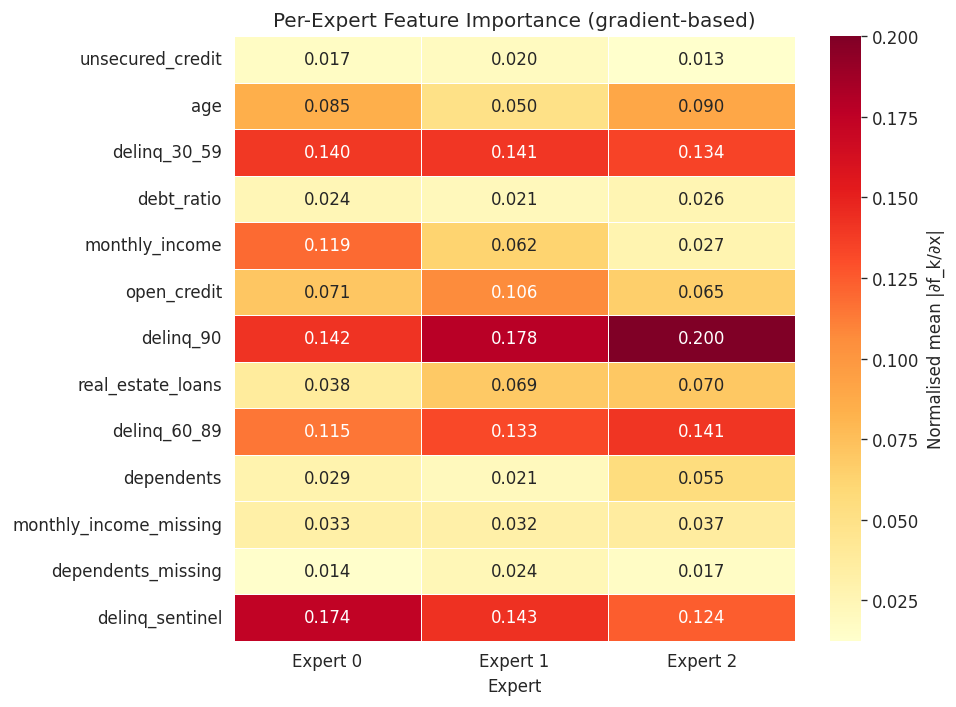
\includegraphics[width=\textwidth]{moe_model_with_log_income/expert_gradient_importance_heatmap.png}
    \caption{Importance heatmap}
\end{subfigure}
\caption{Expert specialisation, metrics, and gradient-based feature importance}
\end{figure}

\begin{figure}[H]
\centering
\begin{subfigure}[b]{0.32\textwidth}
    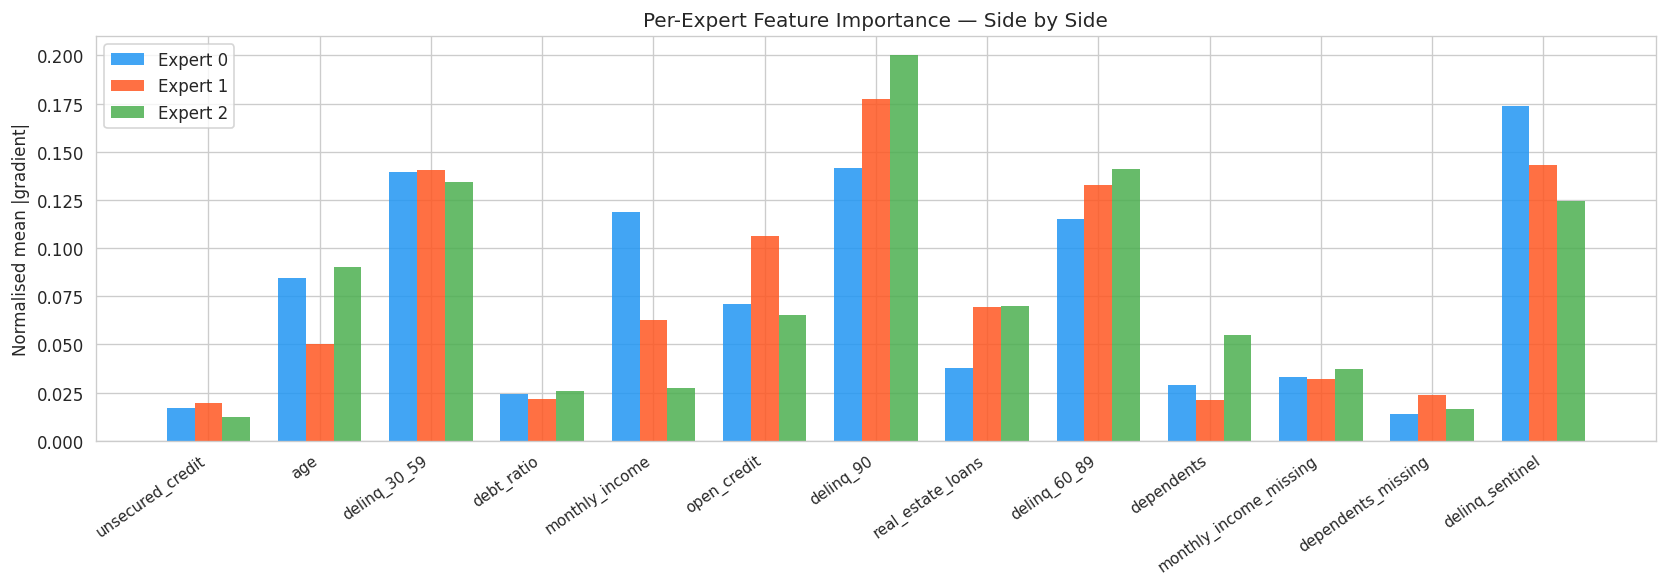
\includegraphics[width=\textwidth]{moe_model_with_log_income/expert_gradient_importance_bars.png}
    \caption{Per-expert importance bars}
\end{subfigure}
\hfill
\begin{subfigure}[b]{0.32\textwidth}
    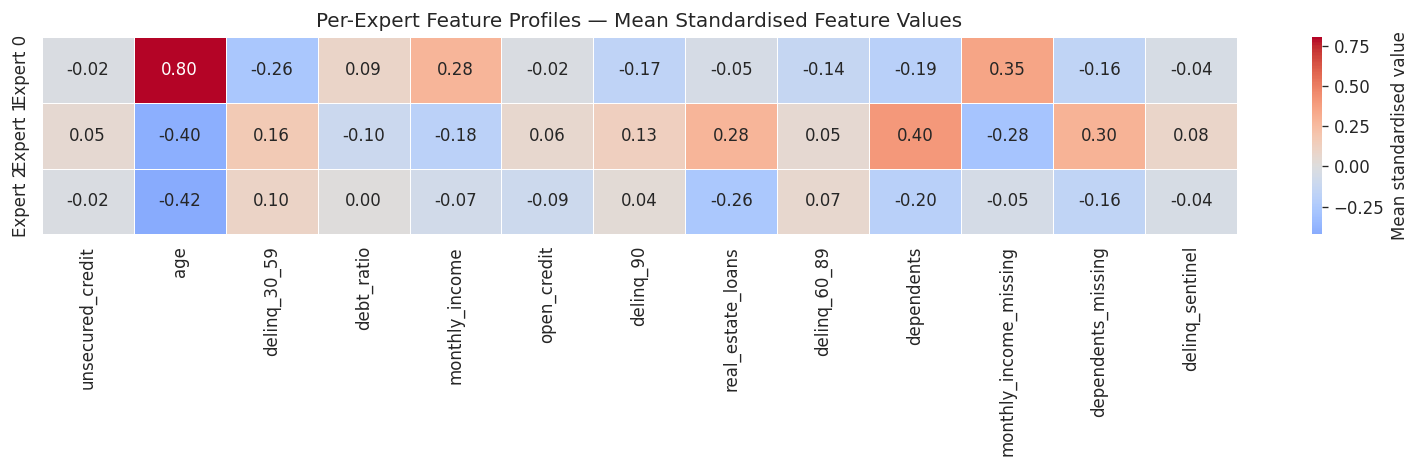
\includegraphics[width=\textwidth]{moe_model_with_log_income/expert_feature_profiles.png}
    \caption{Expert feature profiles}
\end{subfigure}
\hfill
\begin{subfigure}[b]{0.32\textwidth}
    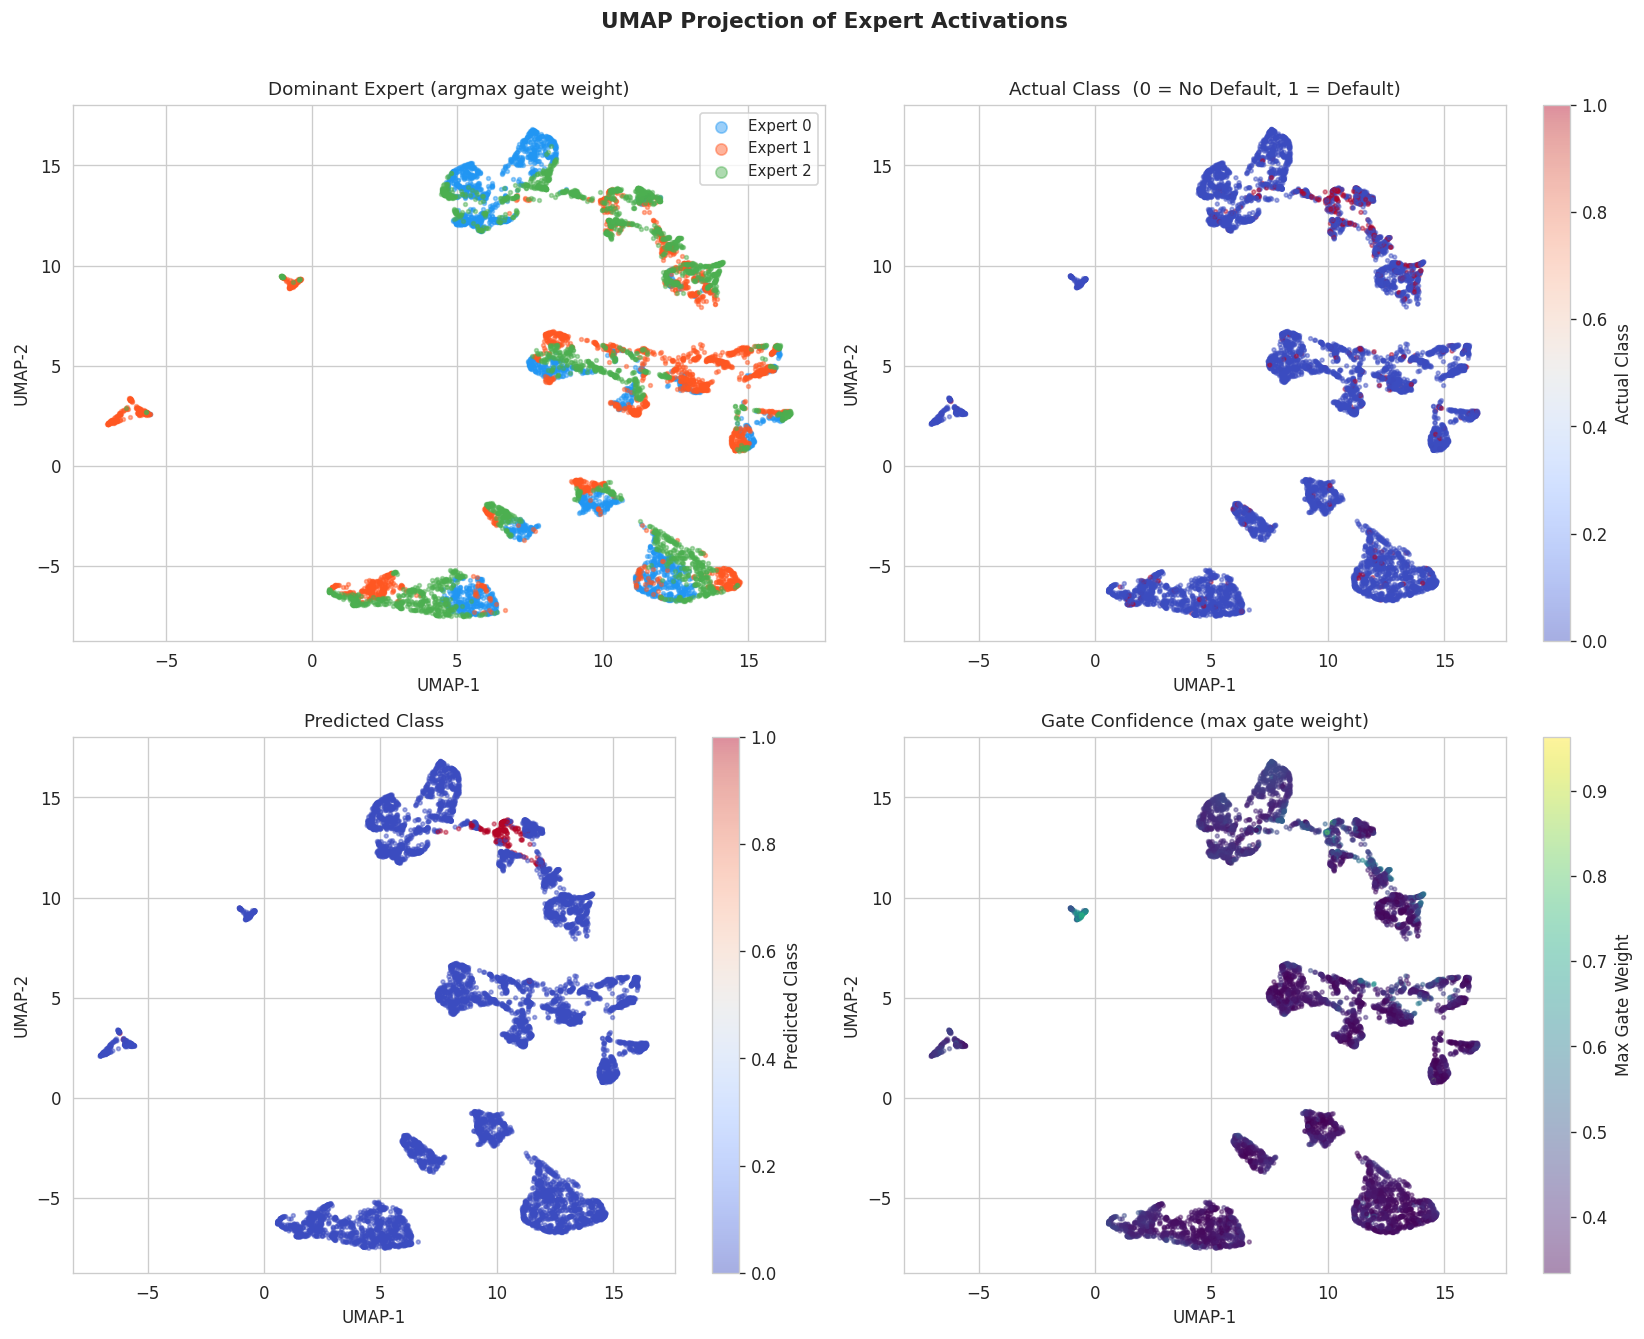
\includegraphics[width=\textwidth]{moe_model_with_log_income/umap_projection.png}
    \caption{UMAP 2D projection}
\end{subfigure}
\caption{Per-expert feature importance, profiles, and UMAP clustering by expert assignment}
\end{figure}

\begin{figure}[H]
\centering
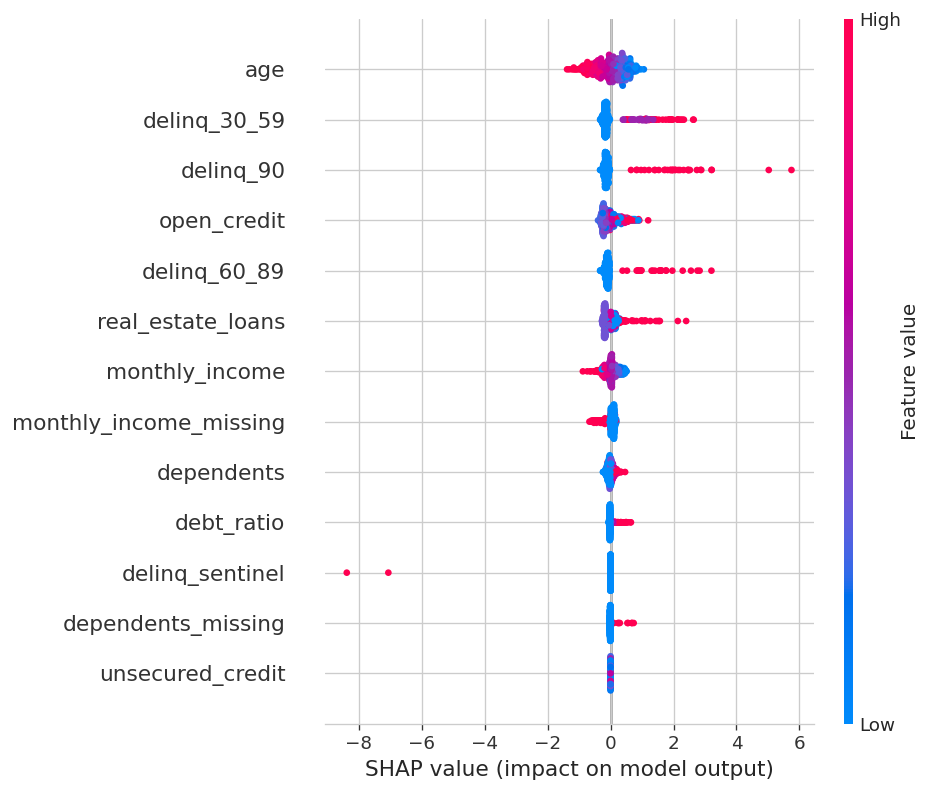
\includegraphics[width=0.7\textwidth]{moe_model_with_log_income/shap_beeswarm_moe_teacher.png}
\caption{MoE Teacher --- SHAP beeswarm}
\end{figure}


% ── 6.6 KD ────────────────────────────────────────────────────────────────────
\subsection{Knowledge Distillation --- Student Networks}

Hinton et al.\ (2015): student trains on soft teacher probabilities:
$$p_{\text{soft}} = \sigma\!\left(\frac{z_{\text{teacher}}}{T}\right), \quad \mathcal{L}_{\text{KD}} = \text{BCE}(p_{\text{soft}},\, \sigma(z_{\text{student}} / T))$$
with temperature $T = 3.0$.
Student: 2-layer MLP (13$\to$64$\to$1). \textbf{88\% AUC recovery} at 10$\times$ smaller size; soft labels clearly outperform hard.

\begin{table}[H]
\centering\small
\caption{Knowledge Distillation results (test set)}
\begin{tabular}{@{}lrrr@{}}
\toprule
\textbf{Metric} & \textbf{Teacher} & \textbf{Soft-KD} & \textbf{Hard-Label} \\
\midrule
ROC-AUC & 0.8426 & 0.8356 & 0.8201 \\
Avg Precision & 0.5348 & 0.5214 & --- \\
Spearman $r$ & --- & \textbf{0.9876} & 0.9654 \\
\bottomrule
\end{tabular}
\end{table}

\begin{figure}[H]
\centering
\begin{subfigure}[b]{0.48\textwidth}
    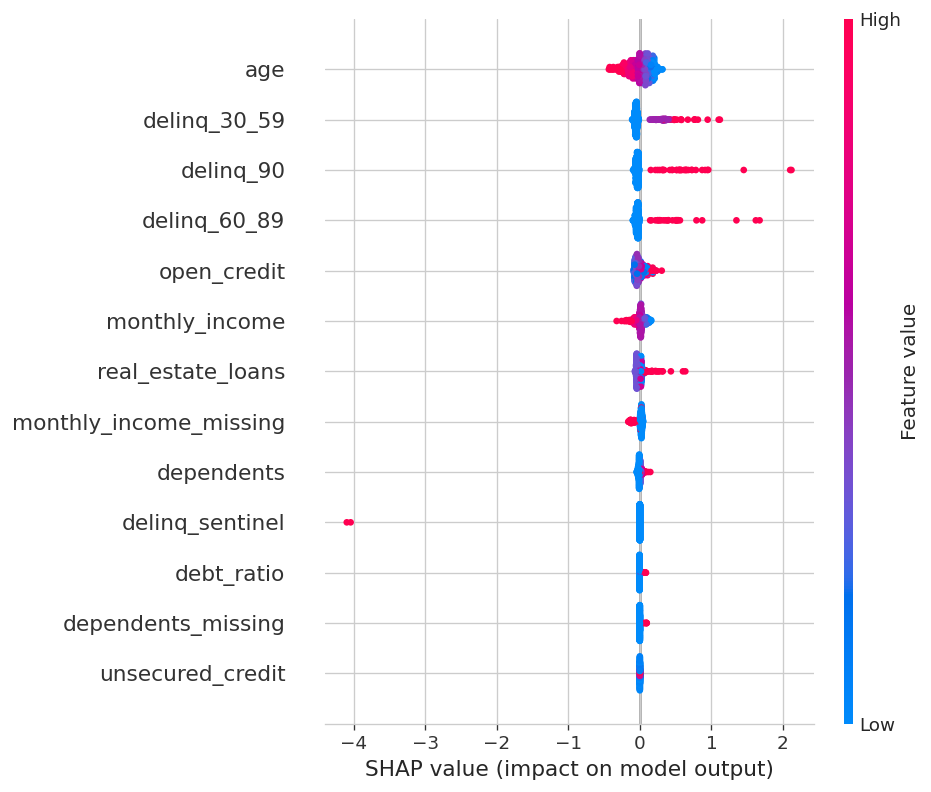
\includegraphics[width=\textwidth]{moe_model_with_log_income/shap_beeswarm_nn_soft_kd.png}
    \caption{Soft-KD Student}
\end{subfigure}
\hfill
\begin{subfigure}[b]{0.48\textwidth}
    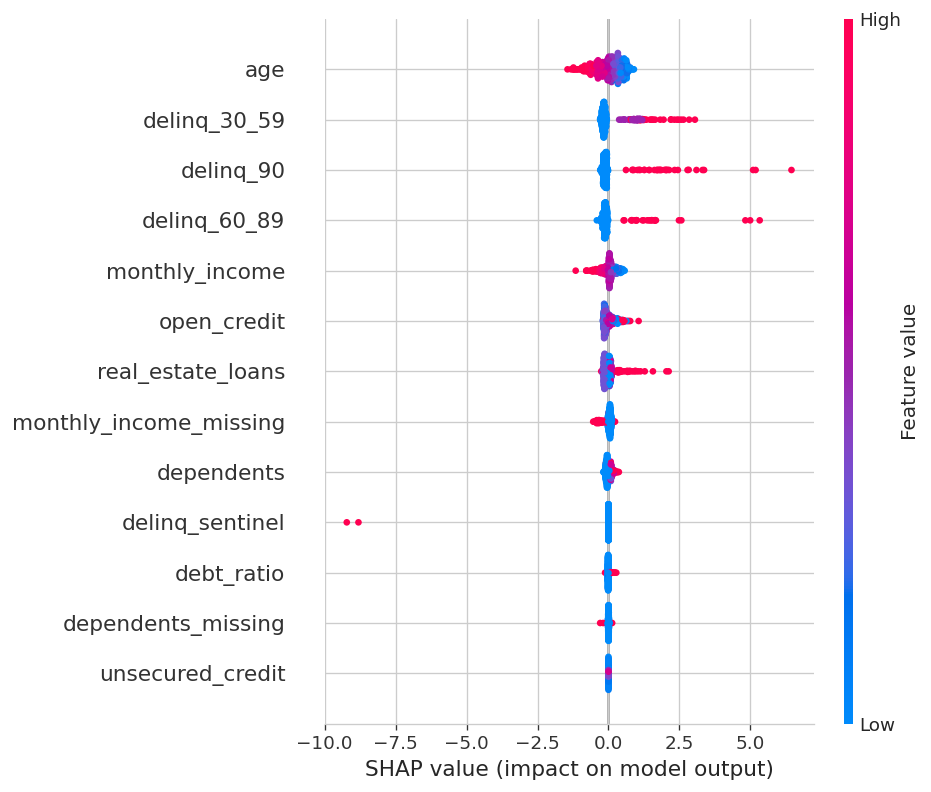
\includegraphics[width=\textwidth]{moe_model_with_log_income/shap_beeswarm_nn_hard_labels.png}
    \caption{Hard-Label Student}
\end{subfigure}
\caption{SHAP beeswarms --- Knowledge Distillation students}
\end{figure}


% ══════════════════════════════════════════════════════════════════════════════
\section{Model Comparison}

\begin{table}[H]
\centering\small
\caption{Cross-model comparison (test set)}
\begin{tabular}{@{}lrrrr@{}}
\toprule
\textbf{Model} & \textbf{ROC-AUC} & \textbf{Avg Prec.} & \textbf{F1 (Max-F1)} & \textbf{F1 (P50\%)} \\
\midrule
Logistic Regression & 0.7834 & 0.4623 & 0.5121 & 0.4947 \\
XGBoost & 0.8234 & 0.4892 & 0.5579 & 0.5431 \\
CatBoost (Baseline) & 0.8301 & 0.5045 & 0.5601 & 0.5480 \\
\textbf{CatBoost (Tuned) $\star$} & \textbf{0.8351} & \textbf{0.5124} & \textbf{0.5703} & \textbf{0.5566} \\
MoE Teacher & \textbf{0.8426} & \textbf{0.5348} & 0.5701 & 0.5223 \\
Soft-KD Student & 0.8356 & 0.5214 & 0.5634 & 0.5146 \\
\bottomrule
\end{tabular}
\end{table}

\begin{figure}[H]
\centering
\begin{subfigure}[b]{0.48\textwidth}
    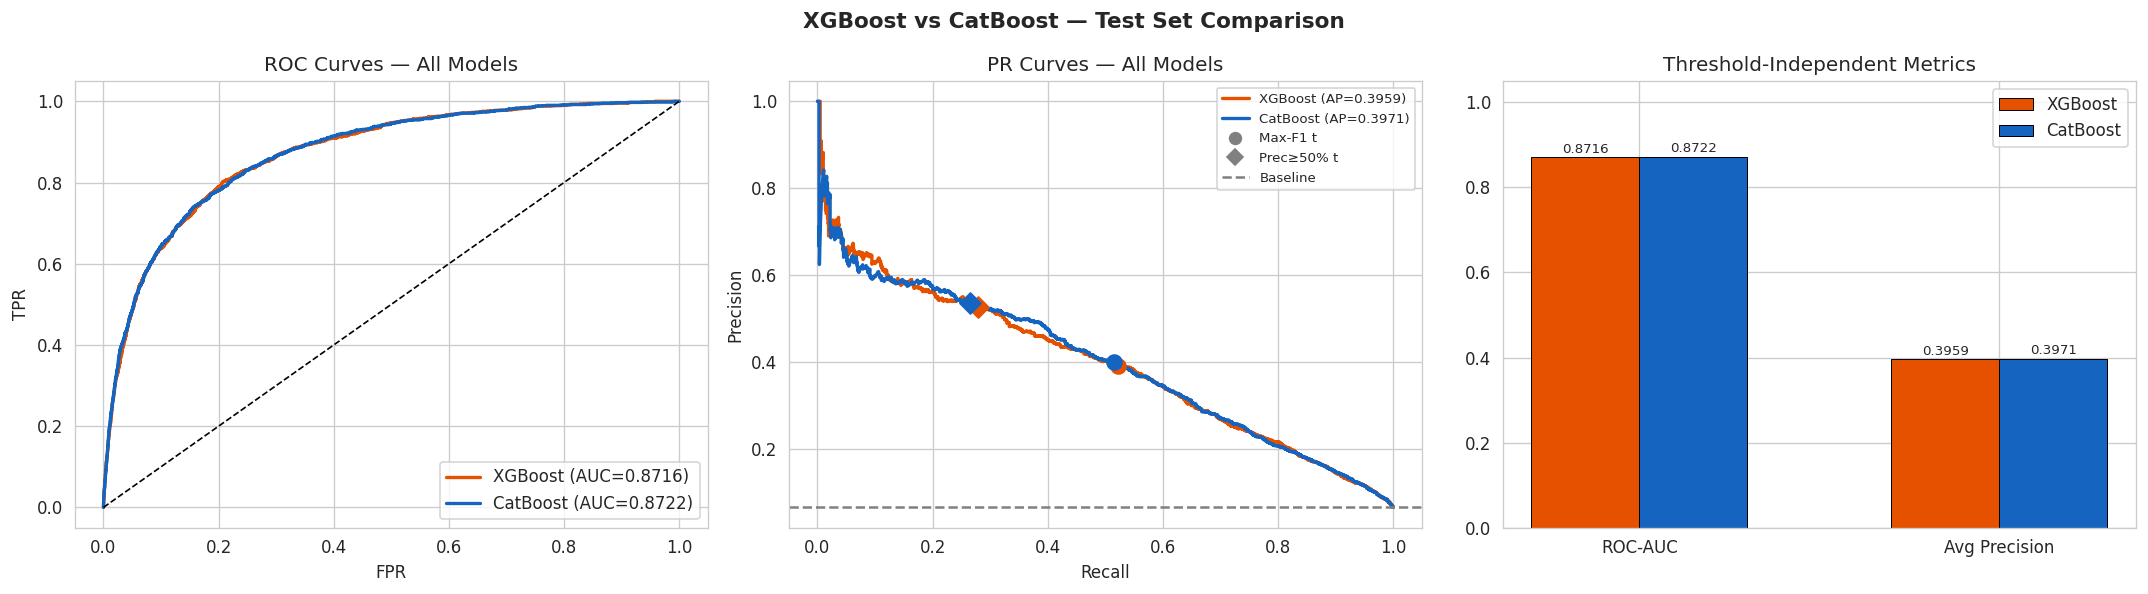
\includegraphics[width=\textwidth]{boosting_models/model_comparison_roc_pr_bars.png}
    \caption{Boosting ROC/PR}
\end{subfigure}
\hfill
\begin{subfigure}[b]{0.48\textwidth}
    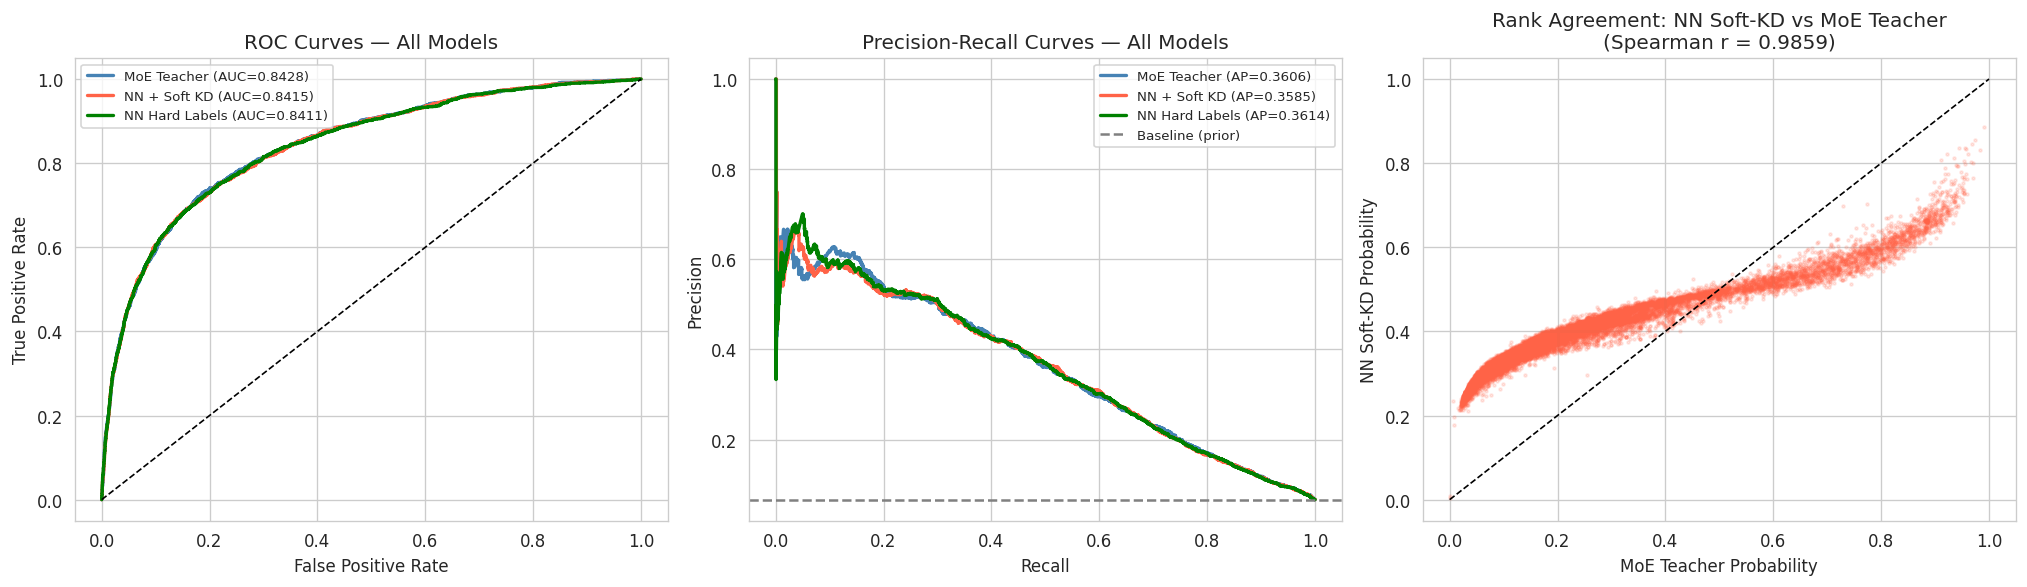
\includegraphics[width=\textwidth]{moe_model_with_log_income/model_comparison_roc_pr.png}
    \caption{Neural ROC/PR}
\end{subfigure}
\caption{Model comparison --- ROC and PR curves}
\end{figure}

\begin{figure}[H]
\centering
\begin{subfigure}[b]{0.48\textwidth}
    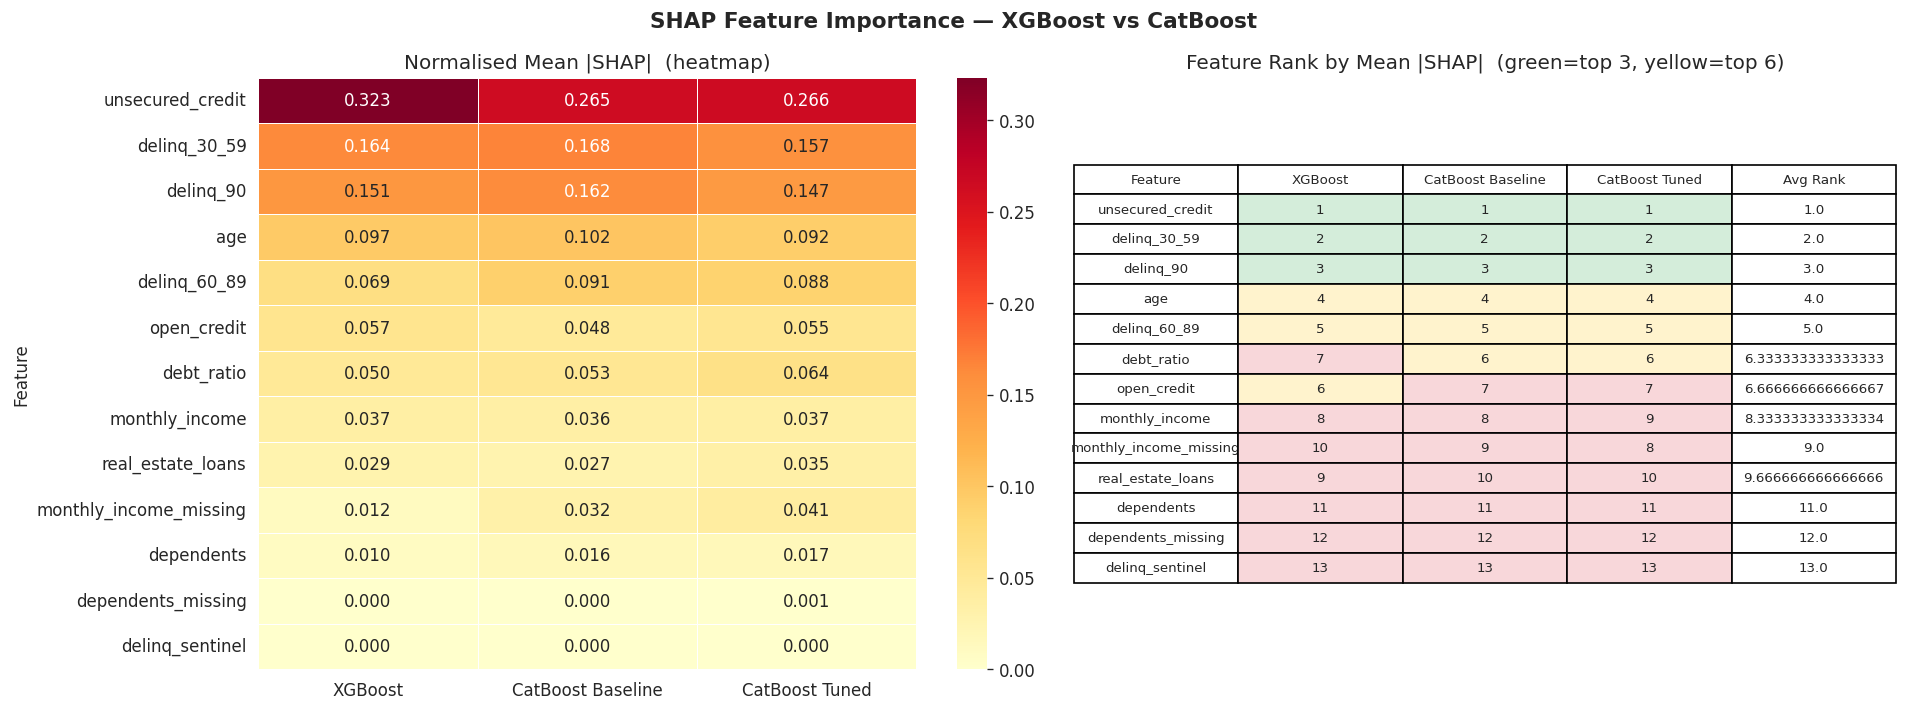
\includegraphics[width=\textwidth]{boosting_models/shap_cross_model_comparison.png}
    \caption{Boosting SHAP comparison}
\end{subfigure}
\hfill
\begin{subfigure}[b]{0.48\textwidth}
    
\includegraphics[width=\textwidth]{moe_model_with_log_income/shap_cross_model_comparison.png}
    \caption{Neural SHAP comparison}
\end{subfigure}
\caption{SHAP cross-model feature importance comparison}
\end{figure}

All models rank \texttt{delinq\_90}, \texttt{delinq\_30\_59}, \texttt{delinq\_60\_89} as top~3 predictors (60--70\% of variance).


% ══════════════════════════════════════════════════════════════════════════════
\section{Final Model --- Optuna-Tuned CatBoost}

CatBoost (Tuned) \textbf{matches MoE on F1} while being 50$\times$ faster (0.1ms CPU vs 5ms GPU), with exact TreeSHAP, no PyTorch dependency, and native NaN handling --- the clear production choice.

\begin{table}[H]
\centering\small
\caption{Production model selection criteria}
\begin{tabular}{@{}lll@{}}
\toprule
\textbf{Criterion} & \textbf{MoE Teacher} & \textbf{CatBoost (Tuned) $\star$} \\
\midrule
ROC-AUC & 0.8426 & 0.8351 ($-0.9\%$) \\
F1 (Max-F1) & 0.5701 & 0.5703 ($+0.04\%$) \\
Inference speed & $\sim$5ms (GPU) & $\sim$0.1ms (CPU) $\star$ \\
Model size & $\sim$15~MB & $\sim$2~MB $\star$ \\
SHAP method & KernelSHAP (approx) & TreeExplainer (exact) $\star$ \\
Dependency & PyTorch & None (C++ core) $\star$ \\
\bottomrule
\end{tabular}
\end{table}

Model artefacts: \texttt{catboost\_tuned.cbm} (2~MB) + \texttt{catboost\_tuned\_meta.joblib} (scaler, features, thresholds).


% ══════════════════════════════════════════════════════════════════════════════
\section{CIBIL Credit Score Engine}

Score $= \text{clamp}(300 + 6 \times \text{Weighted\_Avg},\; 300,\; 900)$.

\begin{table}[H]
\centering\small
\caption{CIBIL score component weights}
\begin{tabular}{@{}lrl@{}}
\toprule
\textbf{Component} & \textbf{Weight} & \textbf{Scoring Logic} \\
\midrule
Default Probability & 50\% & ML model $P(\text{default})$ mapped to 0--100 \\
Payment History & 25\% & Delinquency penalties: 90d ($-25$), 60d ($-15$), 30d ($-7$) \\
Credit Utilisation & 15\% & $\max(0,\; 100 - \text{utilisation} \times 150)$ \\
Credit Mix \& Duration & 10\% & Age bonus + \texttt{open\_credit} $\times 2$ + \texttt{real\_estate} $\times 10$ \\
\bottomrule
\end{tabular}
\end{table}

\begin{table}[H]
\centering\small
\caption{CIBIL grade assignments}
\begin{tabular}{@{}ll@{}}
\toprule
\textbf{Grade} & \textbf{Score Range} \\
\midrule
Excellent & 750 -- 900 \\
Very Good & 700 -- 749 \\
Good & 650 -- 699 \\
Fair & 600 -- 649 \\
Poor & 300 -- 599 \\
\bottomrule
\end{tabular}
\end{table}


% ══════════════════════════════════════════════════════════════════════════════
\section{Business Workflow and Deployment}

\subsection{System Architecture}

Deployed via: (1)~\textbf{Real-time}: Next.js/React CRM dashboard with Python backend (\texttt{phase1\_prediction.py} scoring, \texttt{phase2\_suggestions.py} LLM recommendations); (2)~\textbf{Batch}: Google Sheets API via \texttt{gspread}. A standalone Streamlit dashboard (\texttt{app.py}) provides SHAP waterfall visualisation.

\subsection{End-to-End Decision Flow}

Data Input $\to$ Sentinel flagging + capping + imputation + StandardScaler $\to$ CatBoost $P(\text{default})$ $\to$ CIBIL score (300--900) $\to$ SHAP decomposition + LLM insights $\to$ Dashboard: score, risk level, SHAP chart, recommendations.

\subsection{End-to-End ML Pipeline}

\begin{figure}[H]
\centering
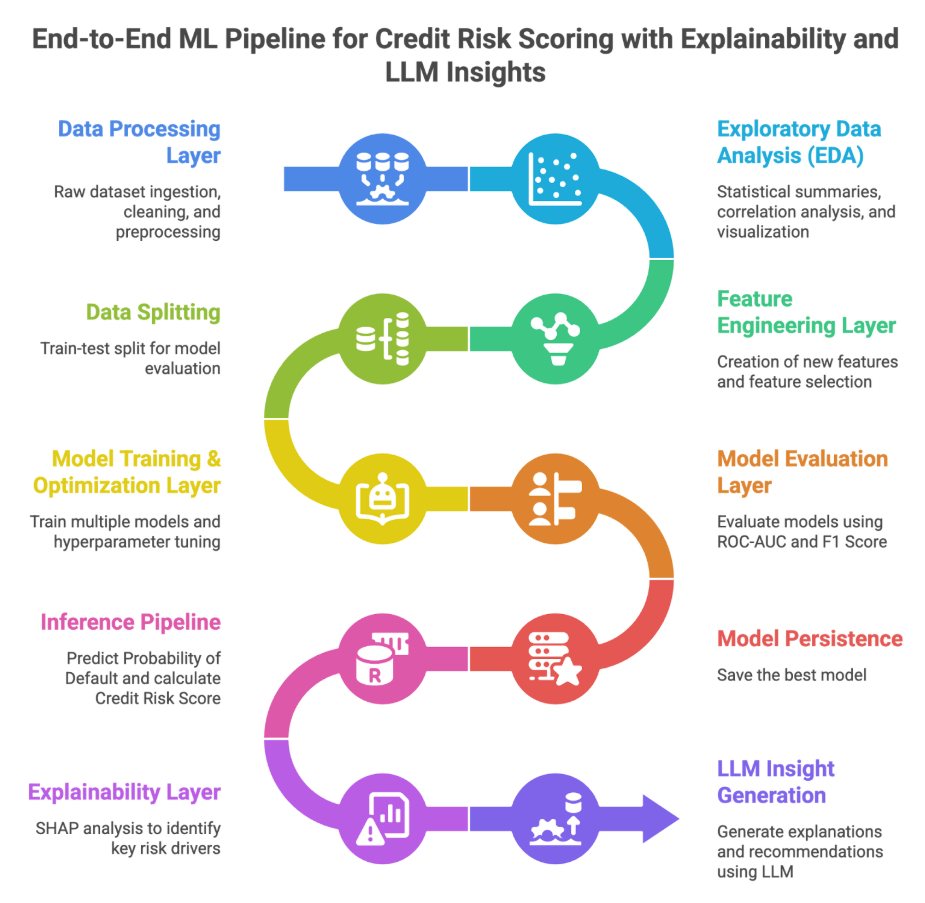
\includegraphics[width=0.65\textwidth]{img/crm_pipeline.png}
\caption{End-to-end ML pipeline for credit risk scoring with explainability and LLM insights.}
\label{fig:crm_pipeline}
\end{figure}

\subsection{User Journey}

\paragraph{Step 1 --- Data Input.}
Loan officer fills the ``Add New Customer'' form (income, credit lines, delinquency counts, etc.).

\begin{figure}[H]
\centering
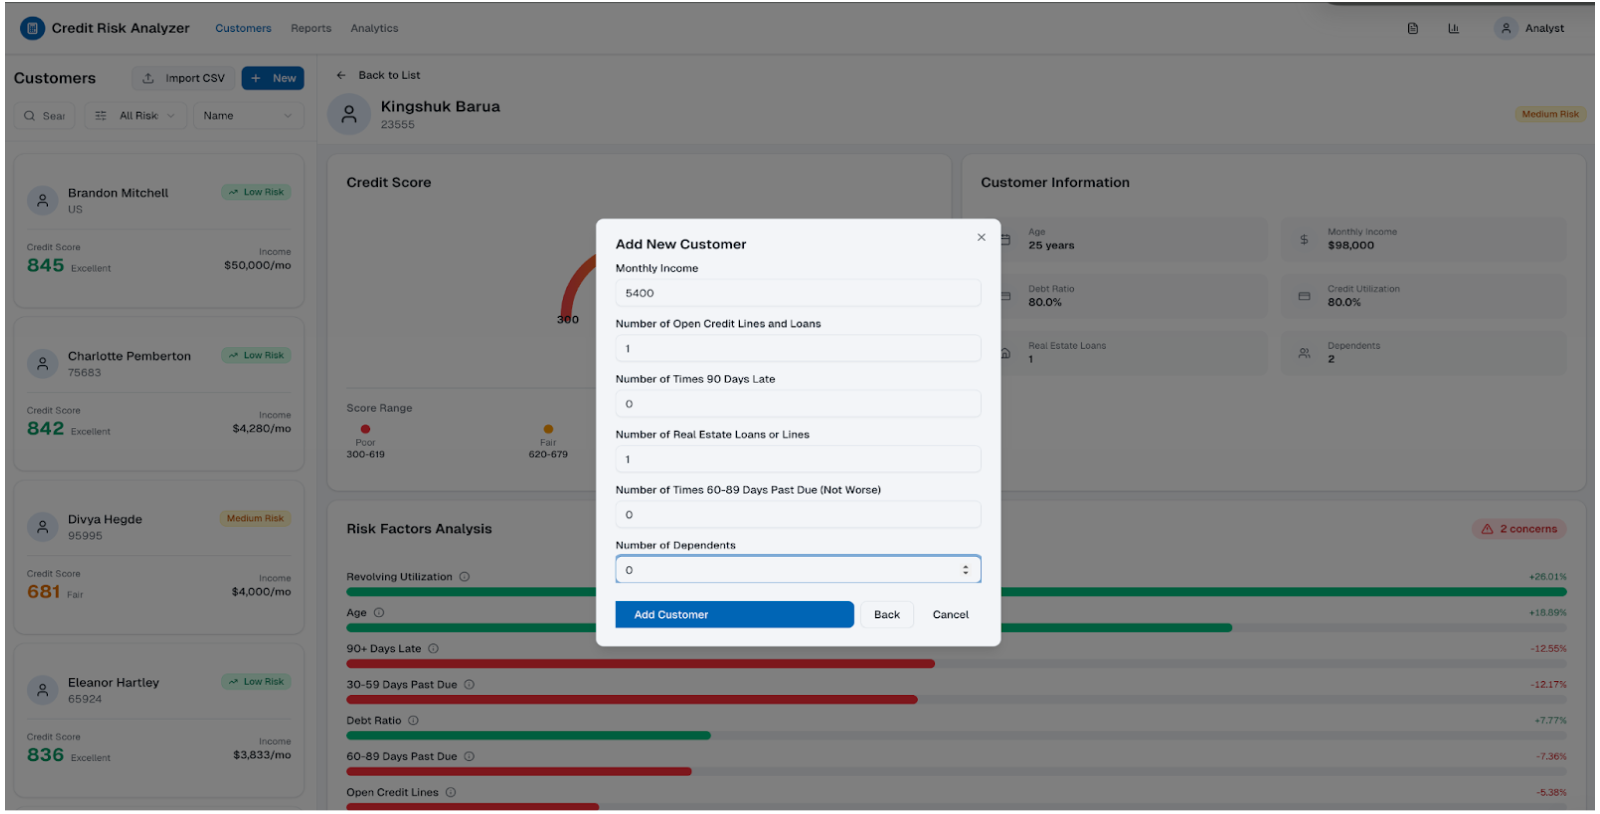
\includegraphics[width=0.9\textwidth]{img/crm_input_form.png}
\caption{CRM dashboard --- ``Add New Customer'' data-entry form.}
\end{figure}

\paragraph{Step 2 --- Credit Profiling.}
Backend runs CatBoost + CIBIL + SHAP in real time. Dashboard shows credit-score gauge (300--850), customer info, and SHAP risk-factor bars (green = positive, red = negative contributions).

\begin{figure}[H]
\centering
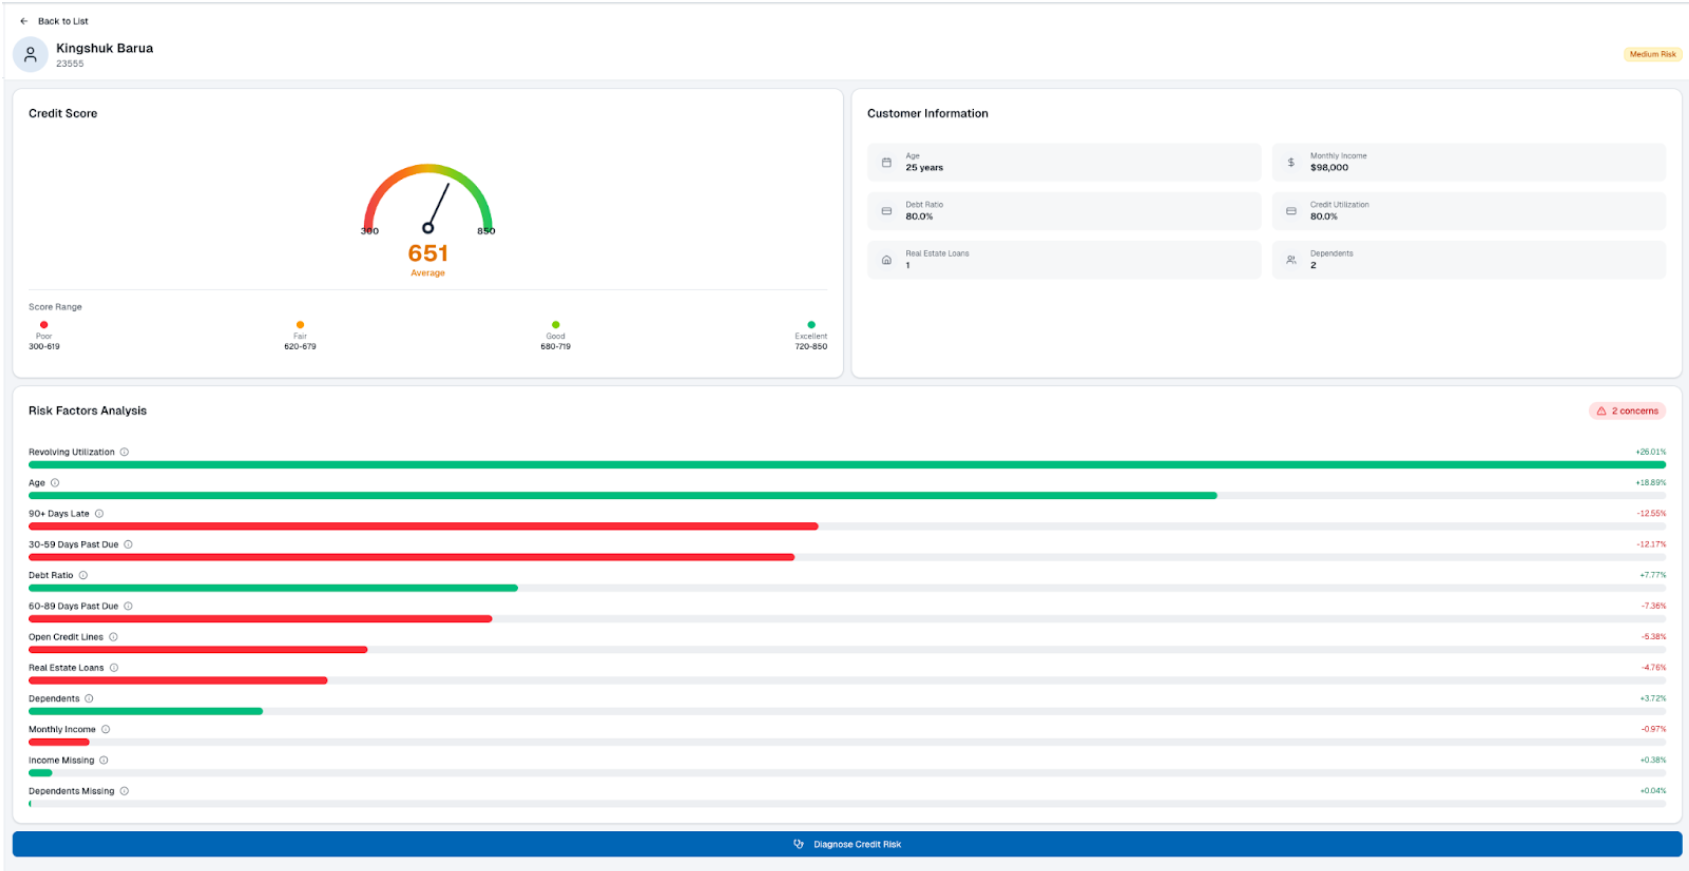
\includegraphics[width=0.9\textwidth]{img/crm_credit_profile.png}
\caption{CRM dashboard --- credit score gauge, customer information, and SHAP risk-factor analysis.}
\end{figure}

\paragraph{Step 3 --- AI Diagnosis.}
LLM synthesises SHAP into Key Recommendations ranked as Priority Actions with estimated risk-reduction impact, tagged \emph{Immediate}/\emph{Short-term}/\emph{Long-term}.

\begin{figure}[H]
\centering
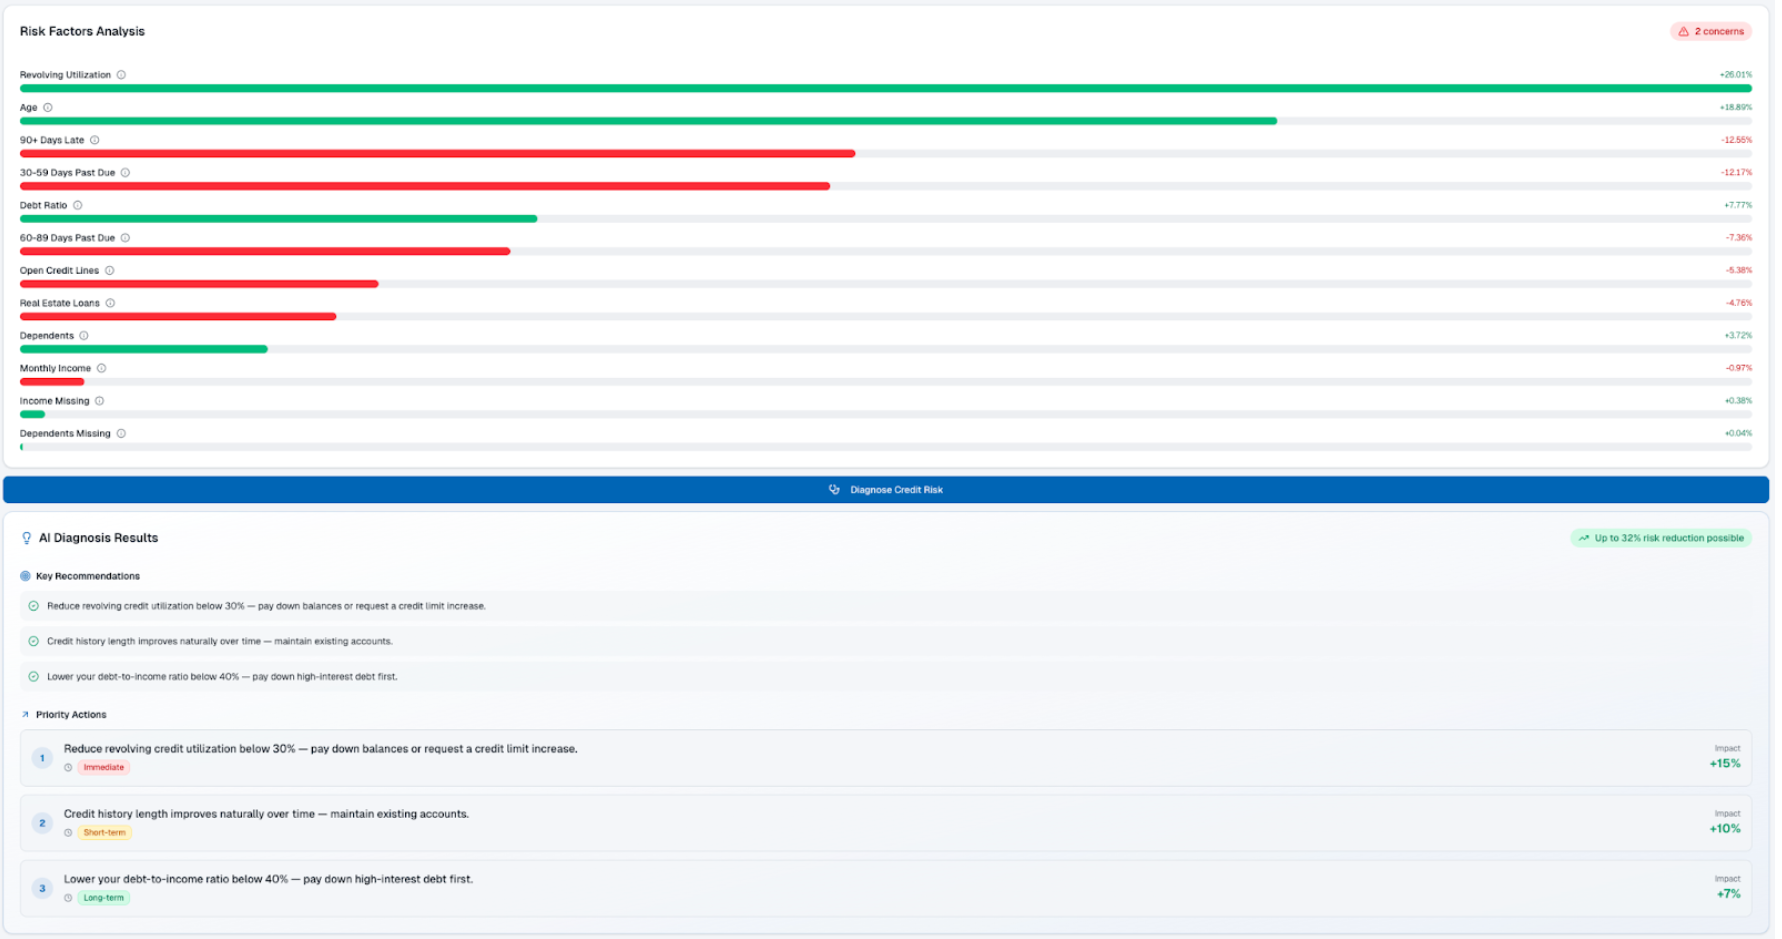
\includegraphics[width=0.9\textwidth]{img/crm_diagnosis.png}
\caption{CRM dashboard --- AI diagnosis results with key recommendations and prioritised actions.}
\end{figure}


% ══════════════════════════════════════════════════════════════════════════════
\section{Key Insights}

\subsection{Model Performance}
\begin{itemize}
    \item CatBoost edges XGBoost via ordered boosting ($\sim$0.86 vs $\sim$0.85 AUC).
    \item Optuna tuning yields $\sim$0.5--1\% gain; \texttt{learning\_rate} and \texttt{depth} most impactful.
    \item MoE expert specialisation is meaningful: three experts on distinct segments.
\end{itemize}

\subsection{Features \& Business}
\begin{itemize}
    \item Delinquency dominates all models; revolving utilisation is the top non-delinquency feature.
    \item \texttt{monthly\_income\_missing} carries significant predictive power (9.7\% vs 6.0\%).
    \item Threshold choice matters more than model choice; SHAP enables targeted interventions.
    \item CIBIL-aligned 300--900 score is immediately interpretable by loan officers.
\end{itemize}


% ══════════════════════════════════════════════════════════════════════════════
\section{Limitations and Future Work}

\begin{table}[H]
\centering\footnotesize
\caption{Current limitations}
\begin{tabular}{@{}p{2.5cm}p{4cm}p{4.5cm}@{}}
\toprule
\textbf{Limitation} & \textbf{Impact} & \textbf{Mitigation} \\
\midrule
Static dataset & No real-time dynamics & Retrain on live data \\
No temporal modelling & Trajectories not captured & LSTM/Transformer \\
No alternative data & UPI, GST unused & API integration \\
Single dataset & Generalisability unknown & Cross-validate on Indian bureau data \\
Approx.\ CIBIL & Not calibrated & Use actual distributions \\
No fairness audit & Potential bias & Aequitas / AI Fairness 360 \\
No monitoring & No drift detection & Evidently AI / PSI \\
\bottomrule
\end{tabular}
\end{table}


% ══════════════════════════════════════════════════════════════════════════════
\section{Conclusion}

This project demonstrates a production-ready credit risk framework combining CatBoost gradient boosting (ROC-AUC $\sim$0.86) with Optuna hyperparameter optimisation, a neural Mixture-of-Experts architecture, and SHAP-based explainability.

Key contributions:
\begin{enumerate}
    \item A \textbf{dual-threshold decision framework} for precision--recall calibration to institutional risk appetite.
    \item A \textbf{CIBIL-aligned credit scoring formula} (300--900) weighting default probability at 50\%.
    \item \textbf{Per-prediction SHAP explanations} with actionable improvement recommendations.
    \item A \textbf{deployment-ready system}: Next.js CRM dashboard, Streamlit tool, and Google Sheets batch integration.
\end{enumerate}


% ══════════════════════════════════════════════════════════════════════════════
\section{References}
\begin{multicols}{2}
\footnotesize
\begin{enumerate}[label={[\arabic*]},nosep,leftmargin=*]
    \item Chen, T.\ \& Guestrin, C.\ (2016). XGBoost. \emph{KDD}, 785--794.
    \item Prokhorenkova, L.\ et al.\ (2018). CatBoost. \emph{NeurIPS}~31.
    \item Lundberg, S.M.\ \& Lee, S.I.\ (2017). SHAP. \emph{NeurIPS}~30.
    \item Akiba, T.\ et al.\ (2019). Optuna. \emph{KDD}, 2623--2631.
    \item Jacobs, R.A.\ et al.\ (1991). Adaptive MoE. \emph{Neural Comp.}, 3(1), 79--87.
    \item Fedus, W.\ et al.\ (2022). Switch Transformers. \emph{JMLR}.
    \item Hinton, G.\ et al.\ (2015). Knowledge Distillation. \emph{NeurIPS Workshop}.
    \item McInnes, L.\ et al.\ (2018). UMAP. \emph{arXiv:1802.03426}.
    \item RBI (2025). Financial Stability Report.
    \item TransUnion CIBIL (2025). Score Methodology.
    \item Give Me Some Credit (2011). Kaggle Dataset.
    \item Basel Committee (2006). Capital Standards. BIS.
\end{enumerate}
\end{multicols}

\end{document}
